\chapter{Results}
\label{ch:results}
	\note{IN PROGRESS}

	\section{Deforestation}
	\label{sec:results_deforestation}

		\subsection{Forest definition}
		\label{subsec:results_forest_definition}
		%TODO appendix graph distribution of the similarity indexes
			\note{Goal:} Our goal was to determine at which canopy cover class the similarity between both layers is greatest to get the subsequent proximate deforestation driver for stable land cover changes optimal by anthropogenic causes by keeping the largest number of pixels from the gfc dataset. We applied the jaccard index for searching the similarity. We grouped our analysis by continental regions americas, asia, africa. Americas accounts for 82 tiles, Asia 86 tiles and Africa 101. We excluded from the analysis all tiles where the initial jaccard index is zero because theses tiles does not contain any tree cover in both tile pairs. This results in 76 Americas , 73 asia and 86 africa. Further we determined the optimal canopy density class for all regions and for single regions by applying the non parametric two and one sided wilcoxon signed rank test. Our initial hypothesis was that the agreement is max between gl30 and hansen when the selected canopy density is between 30 and 100. Because then both datasets should agree by their authors definition of tree cover. The following paragraphs present the results of the analysis for each continental region. 

			\note{Americas:} Figure \ref{fig:jaccard} shows the quartile distribution of the computed jaccard index for each tile pair for each canopy density class over the three continental regions. Plotted on the x-axis is the canopy density class identifier where $JI_0$ accounts for (0,100], $JI_0$ (10,100], $JI_0$ (20,100], and $JI_0$ (30,100]. The y-axis is the corresponding jaccard index between 0 and 1 for the corresponding tile pair where 1 means total agreement and 0 total disagreement. The sample mean highlight by red crosses in the boxplot for the Americas does not change significantly within the different canopy density classes. For all experiments it is approximately 0.62. While the sample median decreases from 0.68 to 0.66 from the first canopy density class the last canopy density class. For the first canopy class the upper 25 \% of the samples have tree cover similarity ranging between approximately 0.8 and 1.0. This behavior can be observed at the other canopy density classes to only the maximal similarity increases slightly from 0.9787 to 0.9798. As the figure \note{appendix} suggests the change of the canopy density have only little impact on the tiles where already the similarity is high for the upper 25 percent. The similarity range of the first two canopy density classes for the lower 25 percent of the samples ranges between approximately 0.0003 and 0.47. Whereas the range for last to canopy classes ranges between 0.0 and 0.5. This suggests that the exclusion of higher canopy densities decreases the similarity at samples where the similarity is already low also shown in figure \note{appendix}. 50 percent of the samples have a jaccard index between approximately 0.5 and 0.8 where here the highest mobility of similarity increase and decrease can be observed. To deduce which canopy density class yield the highest similarity in the distribution overall all samples from americas we applied a wilcoxon test. Tabel \ref{tab:wilcoxontwosided_regions} and \ref{tab:wilcoxontwosided_regions} shows the results from these tests. The two sided test reveals that only the similarity distribution between $JI_0$ and $JI_1$ has a significant (p<0.01) difference in distribution. The other Jaccard Index pairs show now significant difference in distribution. The tree cover similarity distribution of $JC_1$ is significantly greater than $JC_0$ (p<0.005) as the results from the one sided test show in the second table. Therefore the exclusion of canopy densities < 11 fosters the overall agreement between both tree cover datasets. Further the test also reveals that the similarity distribution of $JC_2$ is significantly greater than $JC_1$ (p<0.05) but by the comparison of $JC_1$ and $JC_2$ shows no clear trend in a certain direction. It is to assume that $JC_2$ improves only the tree cover agreement for certain tile pairs and not in general. The same accounts for $JC_3$. For studies targeting Americas it is to recommended to use from the Global Forest Change dataset data which lays within the canopy densities greater than 10 percent.
			\begin{figure}[ht]
				\centering
				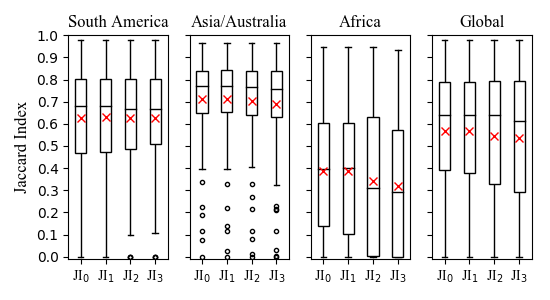
\includegraphics[scale=.91]{img/jaccard}
				\caption[Tree cover similarity distribution of the continental regions]{\textbf{Tree cover similarity distribution over the continental regions:} This boxplot shows the distribution of computed Jaccard Index for each raster image tile pair of GlobeLand30 and Global Forest Change tree cover from 2000. The labels $JI_0$, $JI_1$, $JI_2$, and $JI_3$ on the x-axis account for the canopy density classes (0,100], (10,100], (20,100], and (30,100], respectively. The y-axis is the computed Jaccard Index for the corresponding raster image pair, where 0 is a total disagreement and 1 a total agreement. Red crosses within the $Q_{25}$, $Q_{50}$, and $Q_{75}$ boxes highlight the sample mean. Whiskers are 1.5 times the $IQR$.}
				\label{fig:jaccard}
			\end{figure}
			\begin{table}[ht]
				\centering
				\caption[Two-sided Wilcoxon signed-rank test for regions]{\textbf{Two-sided Wilcoxon signed-rank test for regions:} H$_0$: $\tilde{x_1}=\tilde{x_2}$, The significance is indicated by $p^{*}<0.05$, $p^{**}<0.02$, and $p^{***}<0.01$.}
				\label{tab:wilcoxontwosided_regions}
				\begin{tabular}{llllllllll}
					\hline
					& \multicolumn{3}{c}{Americas} & \multicolumn{3}{c}{Asia} & \multicolumn{3}{c}{Africa} \\
					 & JI$_0$ & JI$_1$ & JI$_2$ & JI$_0$ & JI$_1$ & JI$_2$ & JI$_0$ & JI$_1$ & JI$_2$ \\\hline
					JI$_0$ & - & - & - & - & - & - & - & - & - \\
					JI$_1$ & .00$^{***}$ & - & - & .72 & - & - & .22 & - & - \\
					JI$_2$ & .06 & .36 & - & .00$^{***}$ & .00$^{***}$ & - & .03$^{*}$ & .03$^{*}$  & - \\
					JI$_3$ & .16 & .50 & .60 & .00$^{***}$ & .00$^{***}$ & .00$^{***}$ & .00$^{***}$ & .00$^{***}$ & .00$^{***}$ \\\hline
				\end{tabular}
			\end{table}
			\begin{table}[ht]
				\centering
				\caption[One-sided Wilcoxon signed-rank test for regions]{\textbf{One-sided Wilcoxon signed-rank test for regions:} Columns: H$_0$: $\tilde{x_1}\leq\tilde{x_2}$, Rows: H$_0$: $\tilde{x_1}\geq\tilde{x_2}$, The significance is indicated by $p^{*}<0.05$, $p^{**}<0.025$, $p^{***}<0.01$, and $p^{****}<0.005$.}
				\label{tab:wilcoxononesided_regions}
				\begin{tabular}{lllllllllllll}
					\hline
					& \multicolumn{4}{c}{Americas} & \multicolumn{4}{c}{Asia} & \multicolumn{4}{c}{Africa} \\
					& JI$_0$ & JI$_1$ & JI$_2$ & JI$_3$ & JI$_0$ & JI$_1$ & JI$_2$ & JI$_3$ & JI$_0$ & JI$_1$ & JI$_2$ & JI$_3$ \\\hline
					JI$_0$ & - & .00$^{****}$ & .03$^{*}$ & .08 & - & .64 & 1. & 1. & - & .11 & .98 & 1. \\
					JI$_1$ & 1. & - & .18 & .25 & .36 & - & 1. & 1. & .89 & - & .99 & 1. \\
					JI$_2$ & .97 & .82 & - & .30 & .00$^{****}$ & .00$^{****}$ & - & 1. & .02$^{**}$ & .01$^{**}$ & - & 1. \\
					JI$_3$ & .92 & .75 & .70 & - & .00$^{****}$ & .00$^{****}$ & .00$^{****}$ & - & .00$^{****}$ & .00$^{****}$ & .00$^{****}$ & - \\\hline
				\end{tabular}
			\end{table}
 
			\note{Asia:} As figure \ref{fig:jaccard} suggest does the sample mean is approximately 0.7 for all canopy classes in asia. It decreases slightly at higher canopy density intervals. The median is approximately 0.8 by showing also a slight decrease when the canopy density class is raised. The similarity of the upper 25 percent of the samples is approximately 0.85 and 0.96 and the maximum similarity decreases slightly from 0.9654 to 0.9634 by increasing canopy density interval. This suggests as the appendix figure shows that high ranking tiles are not largely impacted by changes in the canopy density. For Asia the range of the lower 25 percent of the samples is quite large. It ranges between approximately 0.65 and 0.0 and as appendix shows the mobility of the samples show an overall downward trend. The iqr for the first two canopy density classes ranges between 0.65 and 0.85. The exclusion of lower canopy densities have not an large impact on the distribution of tree cover similarity. For last two canopy density classes the range between q1 and q3 is increasing. The exclusion of higher canopy densities leads to overall downwards trend within this intervals figure appendix. For asia the two sided wilcoxon test in table \ref{tab:wilcoxontwosided_regions} reveals that the similarity distribution between every sample pair is significantly different (p<0.01) except the pair of $JI_1$ and $JI_0$. The directional test in table \ref{tab:wilcoxononesided_regions} shows that the overall tree cover agreement of $JI_2$ and $JI_3$ is significantly smaller than $JI_0$ and $JI_1$ (p<0.005). The direction of distribution differences between $JC_0$ and $JC_1$ is not clearly deduce able. This could be explained over a large variability within regional tree cover agreement also a clearer picture could be achieved by applying smaller canopy density exclusion stepping. For studies in asia it is to recommended to use from the Global Forest Change dataset data which lays within the canopy densities greater than 10 percent or the entire data range. Here it must be decided if moving the canopy density threshold below the GlobaLand30 forest cover definition is good trade for increased sample size.

			\note{Africa:} As figure \ref{fig:jaccard} for Africa suggests is the similarity distribution mobility of the samples in Africa at highest. The first two similarity distributions have an comparable mean and median at 0.38 and 0.4. The last two classes show a strong decline in mean and median to approximately 0.33 and 0.3. The mobility of the upper 25 percent of the first two canopy density classes is already quite strong as figure appendix suggests. While the iqr range for $JI_0$ is between 0.15 and 0.6 the range increases for the second $JI_1$ by connecting to more agreement downwards trend. The tile pairs in africa are characterized by a large number of tiles 

			The mean and median is nearly the same for the canopy density classes 1 and 2 with approximately 0.4. Further, the upper 25 percent show a similarity range between 0.6 and 0.94 for both classes. The range of the lower 25 percent changes from 0.15 to 0.1 (lower limit 0.0001) within both classes by an increase of the 50 percent range of the second class. The last two canopy density classes show a strong decline in the median similarity to 0.3. Further the range spreads of the mid 50 percent between 0 and 0.5. The exclusion of lower canopy classes has an large impact on the tree cover agreement in africa. \note{wilcoxon}
			in africa the similarity is largely regional dependent, for continental studies we recommend to use the full range of the hansen dataset or max exclude till 10 percent canopy density

			\note{Comparison between regions:} Asia shows the highest tree cover similarity over all regions followed by the Americas. Africa the tree cover agreement within the tile pairs is poorest. The iqr is for asia at lowest followed by americas and africa with the widest range in the mid 50 percent interval. At the upper 25 percent america and asia show no large mobility at a change of canopy density. These high agreement tiles highlight core forest zones where only a few number of pixels has lower canopy density values which could be excluded. Further this highlights that within these zones both datasets yield high certainty about the forest cover. Africa has only small core tropical forest zones and there the change of canopy density has also an strong impact on the overall similarity which is proved by the high mobility of samples within the upper 25 percent. Therefore Africa shows the greatest regional dependency of tree cover similarity. The same effect is also for Americas and Asia observable but not as strong as in africa. \note{Wilcoxon}

			\note{Whats the result for all regions:}
			\begin{table}[ht]
				\centering
				\caption[Two-sided Wilcoxon signed-rank test for all samples]{\textbf{Two-sided Wilcoxon signed-rank test for all samples:} H$_0$: $\tilde{x_1}=\tilde{x_2}$, The significance is indicated by $p^{*}<0.05$, $p^{**}<0.02$, and $p^{***}<0.01$.}
				\label{tab:wilcoxontwosided_all}
				\begin{tabular}{llll}
					\hline
					& JI$_0$ & JI$_1$ & JI$_2$ \\\hline
					JI$_0$ & - & - & - \\
					JI$_1$ & .00$^{***}$ & - & - \\
					JI$_2$ & .08 & .02$^{**}$ & - \\
					JI$_3$ & .00$^{***}$ & .00$^{***}$ & .00$^{***}$ \\\hline
				\end{tabular}
			\end{table}
			\begin{table}[ht]
				\centering
				\caption[One-sided Wilcoxon signed-rank test fro all samples]{\textbf{One-sided Wilcoxon signed-rank test for all samples:} Columns: H$_0$: $\tilde{x_1}\leq\tilde{x_2}$, Rows: H$_0$: $\tilde{x_1}\geq\tilde{x_2}$, The significance is indicated by $p^{*}<0.05$, $p^{**}<0.025$, $p^{***}<0.01$, and $p^{****}<0.005$.}
				\label{tab:wilcoxononesided_all}
				\begin{tabular}{lllll}
					\hline
					& JI$_0$ & JI$_1$ & JI$_2$ & JI$_3$ \\\hline
					JI$_0$ & - & .00$^{****}$ & .96 & 1. \\
					JI$_1$ & 1. & - & .99 & 1. \\
					JI$_2$ & .04$^{*}$ & .01$^{***}$ & - & 1. \\
					JI$_3$ & .00$^{****}$ & .00$^{****}$ & .00$^{****}$ & - \\\hline
				\end{tabular}
			\end{table}

		\subsection{Tree cover and deforestation}
		\label{subsec:results_tree_cover_and_deforestation}

		\subsection{Proximate deforestation driver}
		\label{subsec:results_proxy_deforestation_driver}

		\subsection{Accuracy assessment}
		\label{subsec:results_accuracy_assessment}
			\begin{table}[ht]
				\centering
				\caption[Accuracy assessment]{Confusion matrix for accuracy assessment}
				\label{tab:accuracy}
				\begin{tabular}{llrrrrrrrrrrrr}
					\hline
					& & \multicolumn{9}{c}{Reference} & & & \\
					& Cls & 10 & 20 & 25 & 30 & 40 & 50 & 60 & 80 & 90 & Tot & UAc & Om \\\hline
					\multirow{9}{*}{\STAB{\rotatebox[origin=c]{90}{Prediction}}}
					& 10 & 732 & 38 & 62 & 15 & 16 & 2 & 3 & 5 & 0 & 873 & .84 & .16 \\ 
					& 20 & 42 & 751 & 57 & 189 & 31 & 12 & 0 & 17 & 4 & 1103 & .68 & .32 \\ 
					& 25 & 29 & 202 & 1155 & 173 & 22 & 10 & 5 & 11 & 4 & 1611 & .72 & .28 \\ 
					& 30 & 36 & 187 & 32 & 1466 & 73 & 21 & 0 & 17 & 0 & 1832 & .80 & .20 \\ 
					& 40 & 14 & 21 & 4 & 41 & 352 & 1 & 1 & 2 & 1 & 437 & .81 & .19 \\ 
					& 50 & 0 & 5 & 3 & 10 & 4 & 50 & 0 & 1 & 0 & 73 & .68 & .32 \\ 
					& 60 & 2 & 1 & 0 & 3 & 0 & 2 & 18 & 2 & 0 & 28 & .64 & .36 \\ 
					& 80 & 3 & 4 & 0 & 1 & 1 & 1 & 0 & 50 & 0 & 60 & .83 & .17 \\ 
					& 90 & 0 & 0 & 0 & 1 & 0 & 0 & 0 & 3 & 5 & 9 & .56 & .44 \\\hline 
					& Tot & 858 & 1209 & 1313 & 1899 & 499 & 99 & 27 & 108 & 14 & 6026 & & \\
					& PAc & .85 & .62 & .88 & .77 & .71 & .51 & .67 & .46 & .36 & & \multicolumn{2}{r}{OvAc} \\
					& Com & .15 & .38 & .12 & .23 & .29 & .49 & .33 & .54 & .64 & & \multicolumn{2}{r}{.75} \\ \hline
				\end{tabular}
			\end{table}

	\section{Emissions}

	\section{Ecosystem service values}




%%%%%%% TABLE AND FIGURES

%			\begin{table}[ht]
%				\centering
%				\caption[Deforestation driver]{Absolute in km$^2$}
%				\label{tab:driver_tab}
%				\begin{tabular}{lcllrrr}
%					Class & Code & Type & & Americas & Asia & Africa \\\hline
%					\multirow{4}{*}{Agriculture} & \multirow{2}{*}{10} & \multirow{2}{*}{Cropland} & rel. & 24.37 & 18.37 & 25.01 \\
%					& & & abs. & 95908 & 38719 & 44368 \\
%					& \multirow{2}{*}{30} & \multirow{2}{*}{Grassland} & rel. & 46.19 & 8.41 & 50.46 \\
%					& & & abs. & 181781 & 17726 & 89516 \\
%					\multirow{4}{*}{Forestry/Plantations} & \multirow{2}{*}{25} & \multirow{2}{*}{Regrowth} & rel. & 14.40 & 70.27 & 18.61 \\
%					& & & abs. & 56671 & 148111 & 33014 \\
%					& \multirow{2}{*}{40} & \multirow{2}{*}{Shrubland} & rel. & 12.69 & 1.11 & 3.77 \\
%					& & & abs. & 49941 & 2340 & 6688 \\
%					\multirow{4}{*}{Urban/Mining} & \multirow{2}{*}{80} & \multirow{2}{*}{Artificial} & rel. & 0.41 & 0.46 & 0.71 \\
%					& & & abs. & 1614 & 970 & 1260 \\
%					& \multirow{2}{*}{90} & \multirow{2}{*}{Bareland} & rel. & 0.10 & 0.03 & 0.09 \\
%					& & & abs. & 394 & 63 & 160 \\
%					\multirow{4}{*}{Natural} & \multirow{2}{*}{50} & \multirow{2}{*}{Wetland} & rel. & 1.50 & 0.97 & 1.23 \\
%					& & & abs. & 5903 & 2045 & 2182 \\
%					& \multirow{2}{*}{60} & \multirow{2}{*}{Water} & rel. & 0.32 & 0.38 & 0.13 \\
%					& & & abs. & 1259 & 801 & 231 \\\hline
%					\multicolumn{3}{c}{\multirow{2}{*}{Forest loss}} & rel. & 3.87 & 4.68 & 1.69 \\
%					& & & abs. & 393550 & 210774 & 177400 \\
%					\multicolumn{3}{c}{Forest cover} & abs. & 10223187 & 4457940 & 10496591 \\\hline
%				\end{tabular}
%			\end{table}

% LATIN AMERICA
%			\begin{figure}[ht]
%				\centering
%				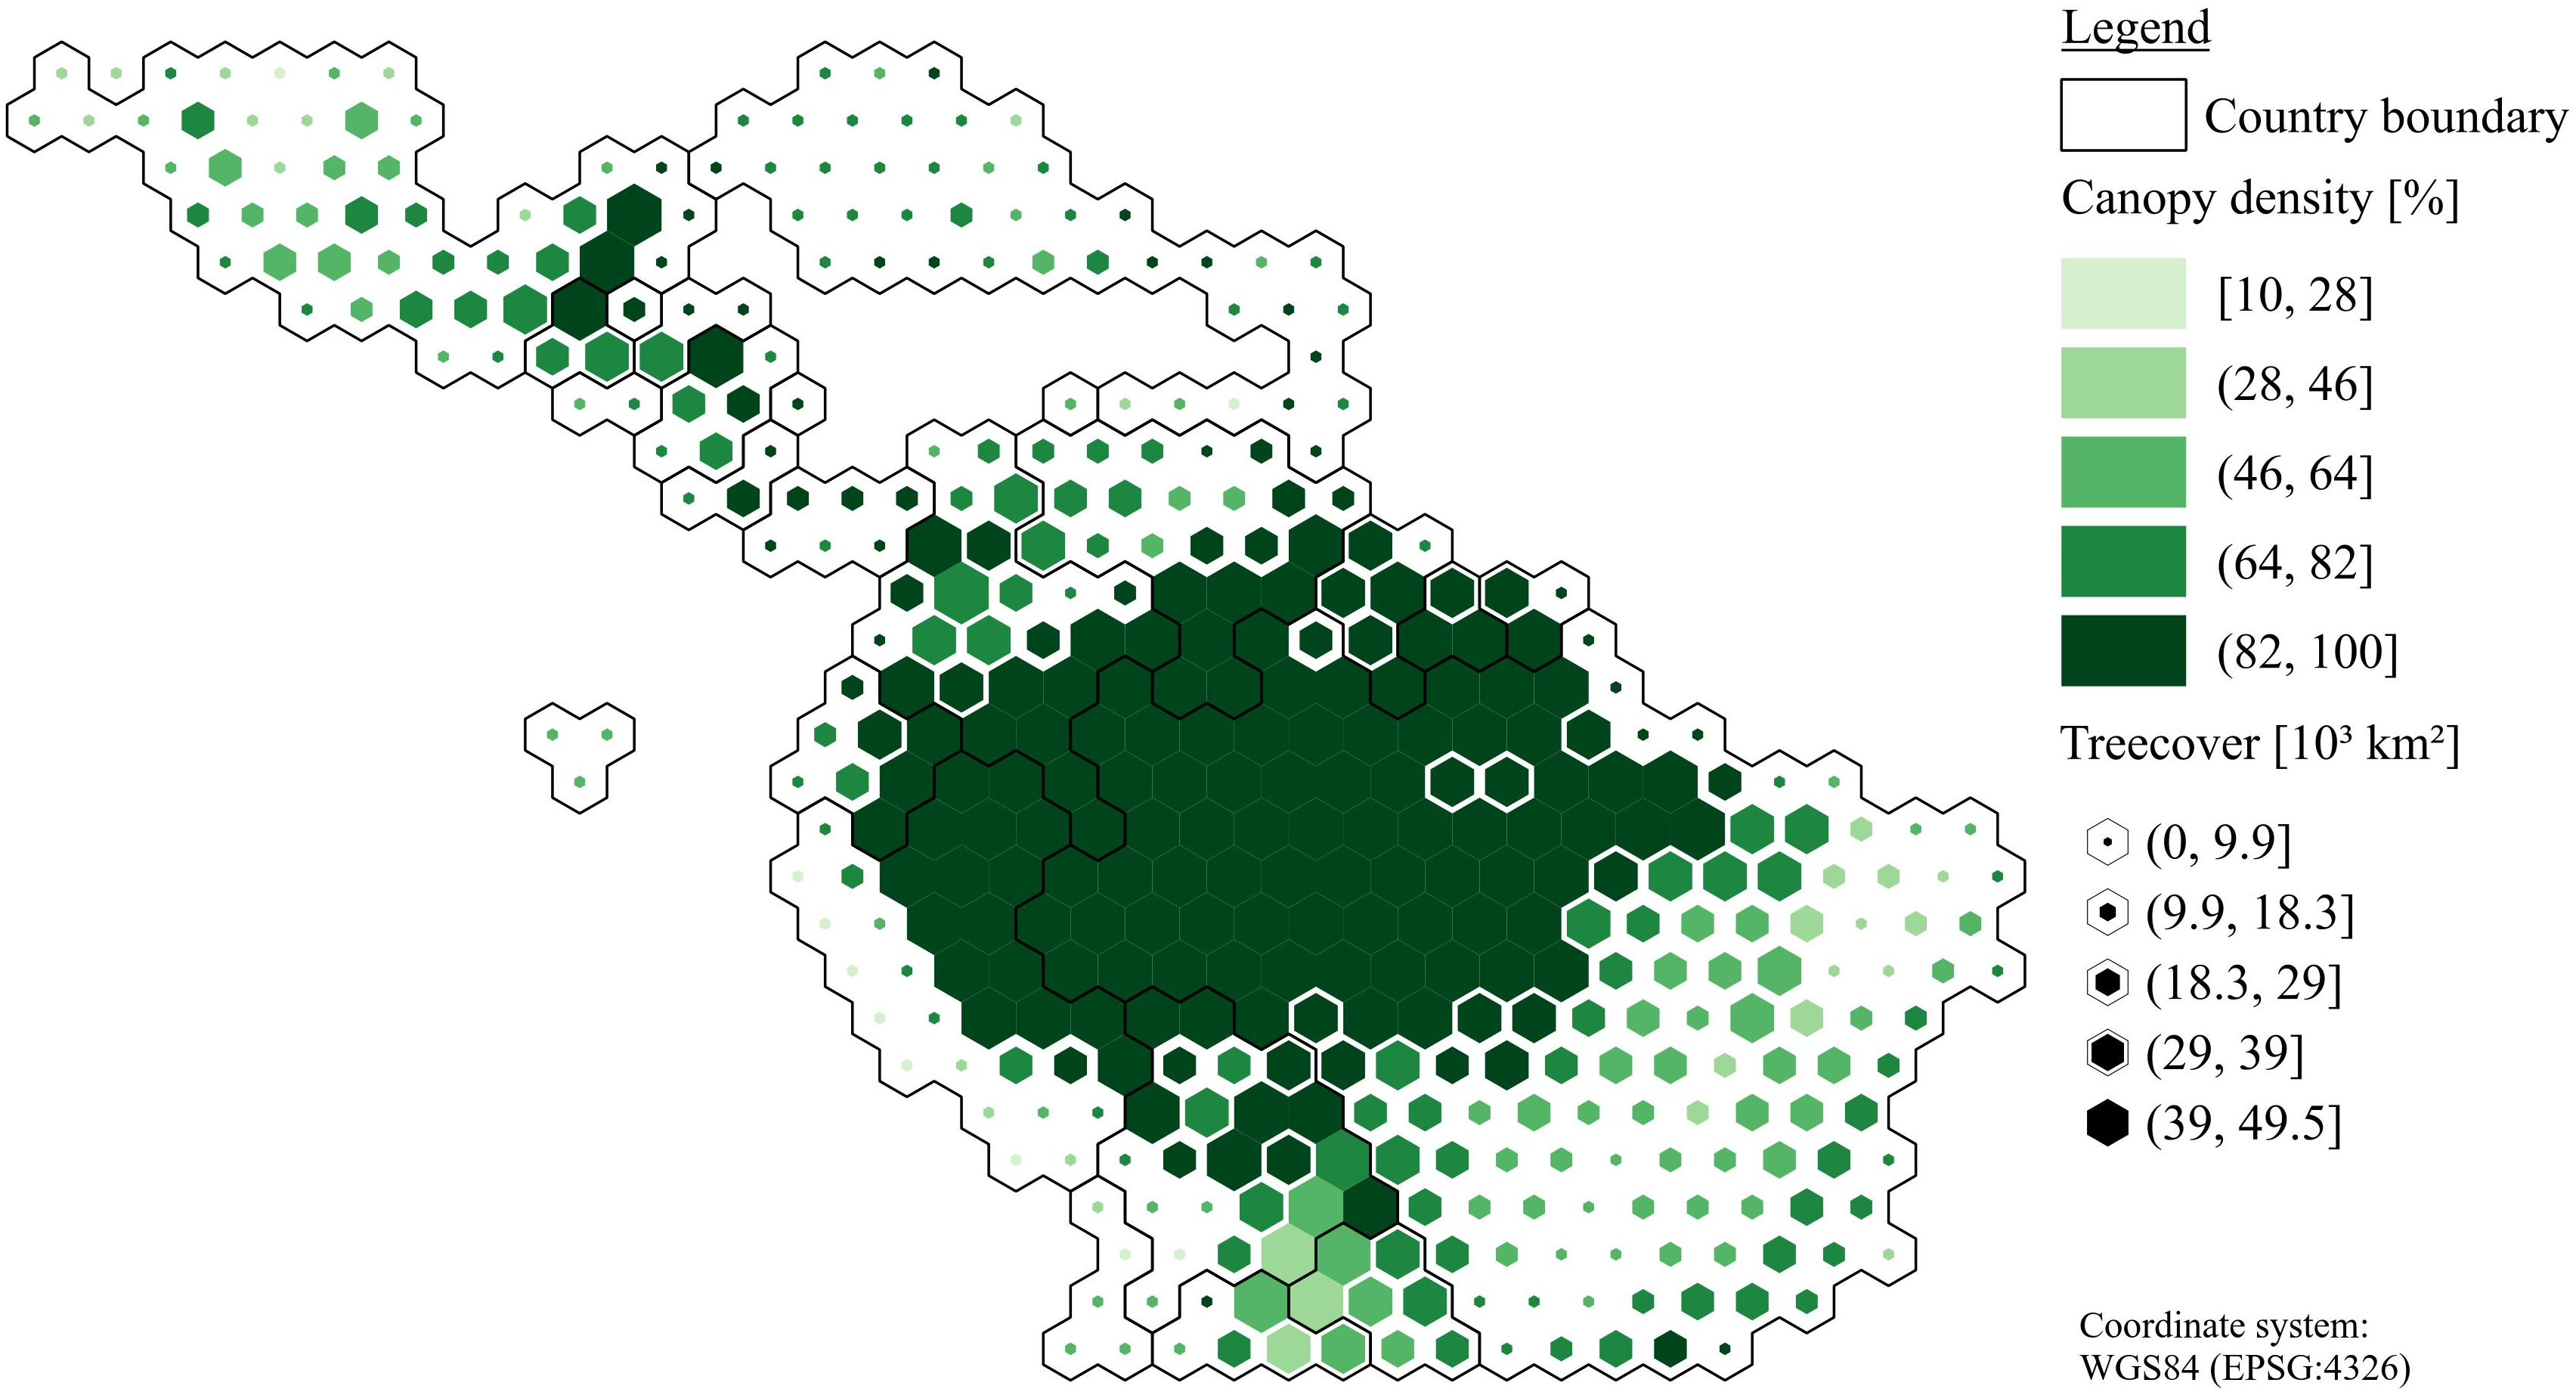
\includegraphics[scale=1]{img/americas_treecover_frameless}
%				\caption[Ecosystem service values]{}
%				\label{fig:americascover}
%			\end{figure}
%			\begin{figure}[ht]
%				\centering
%				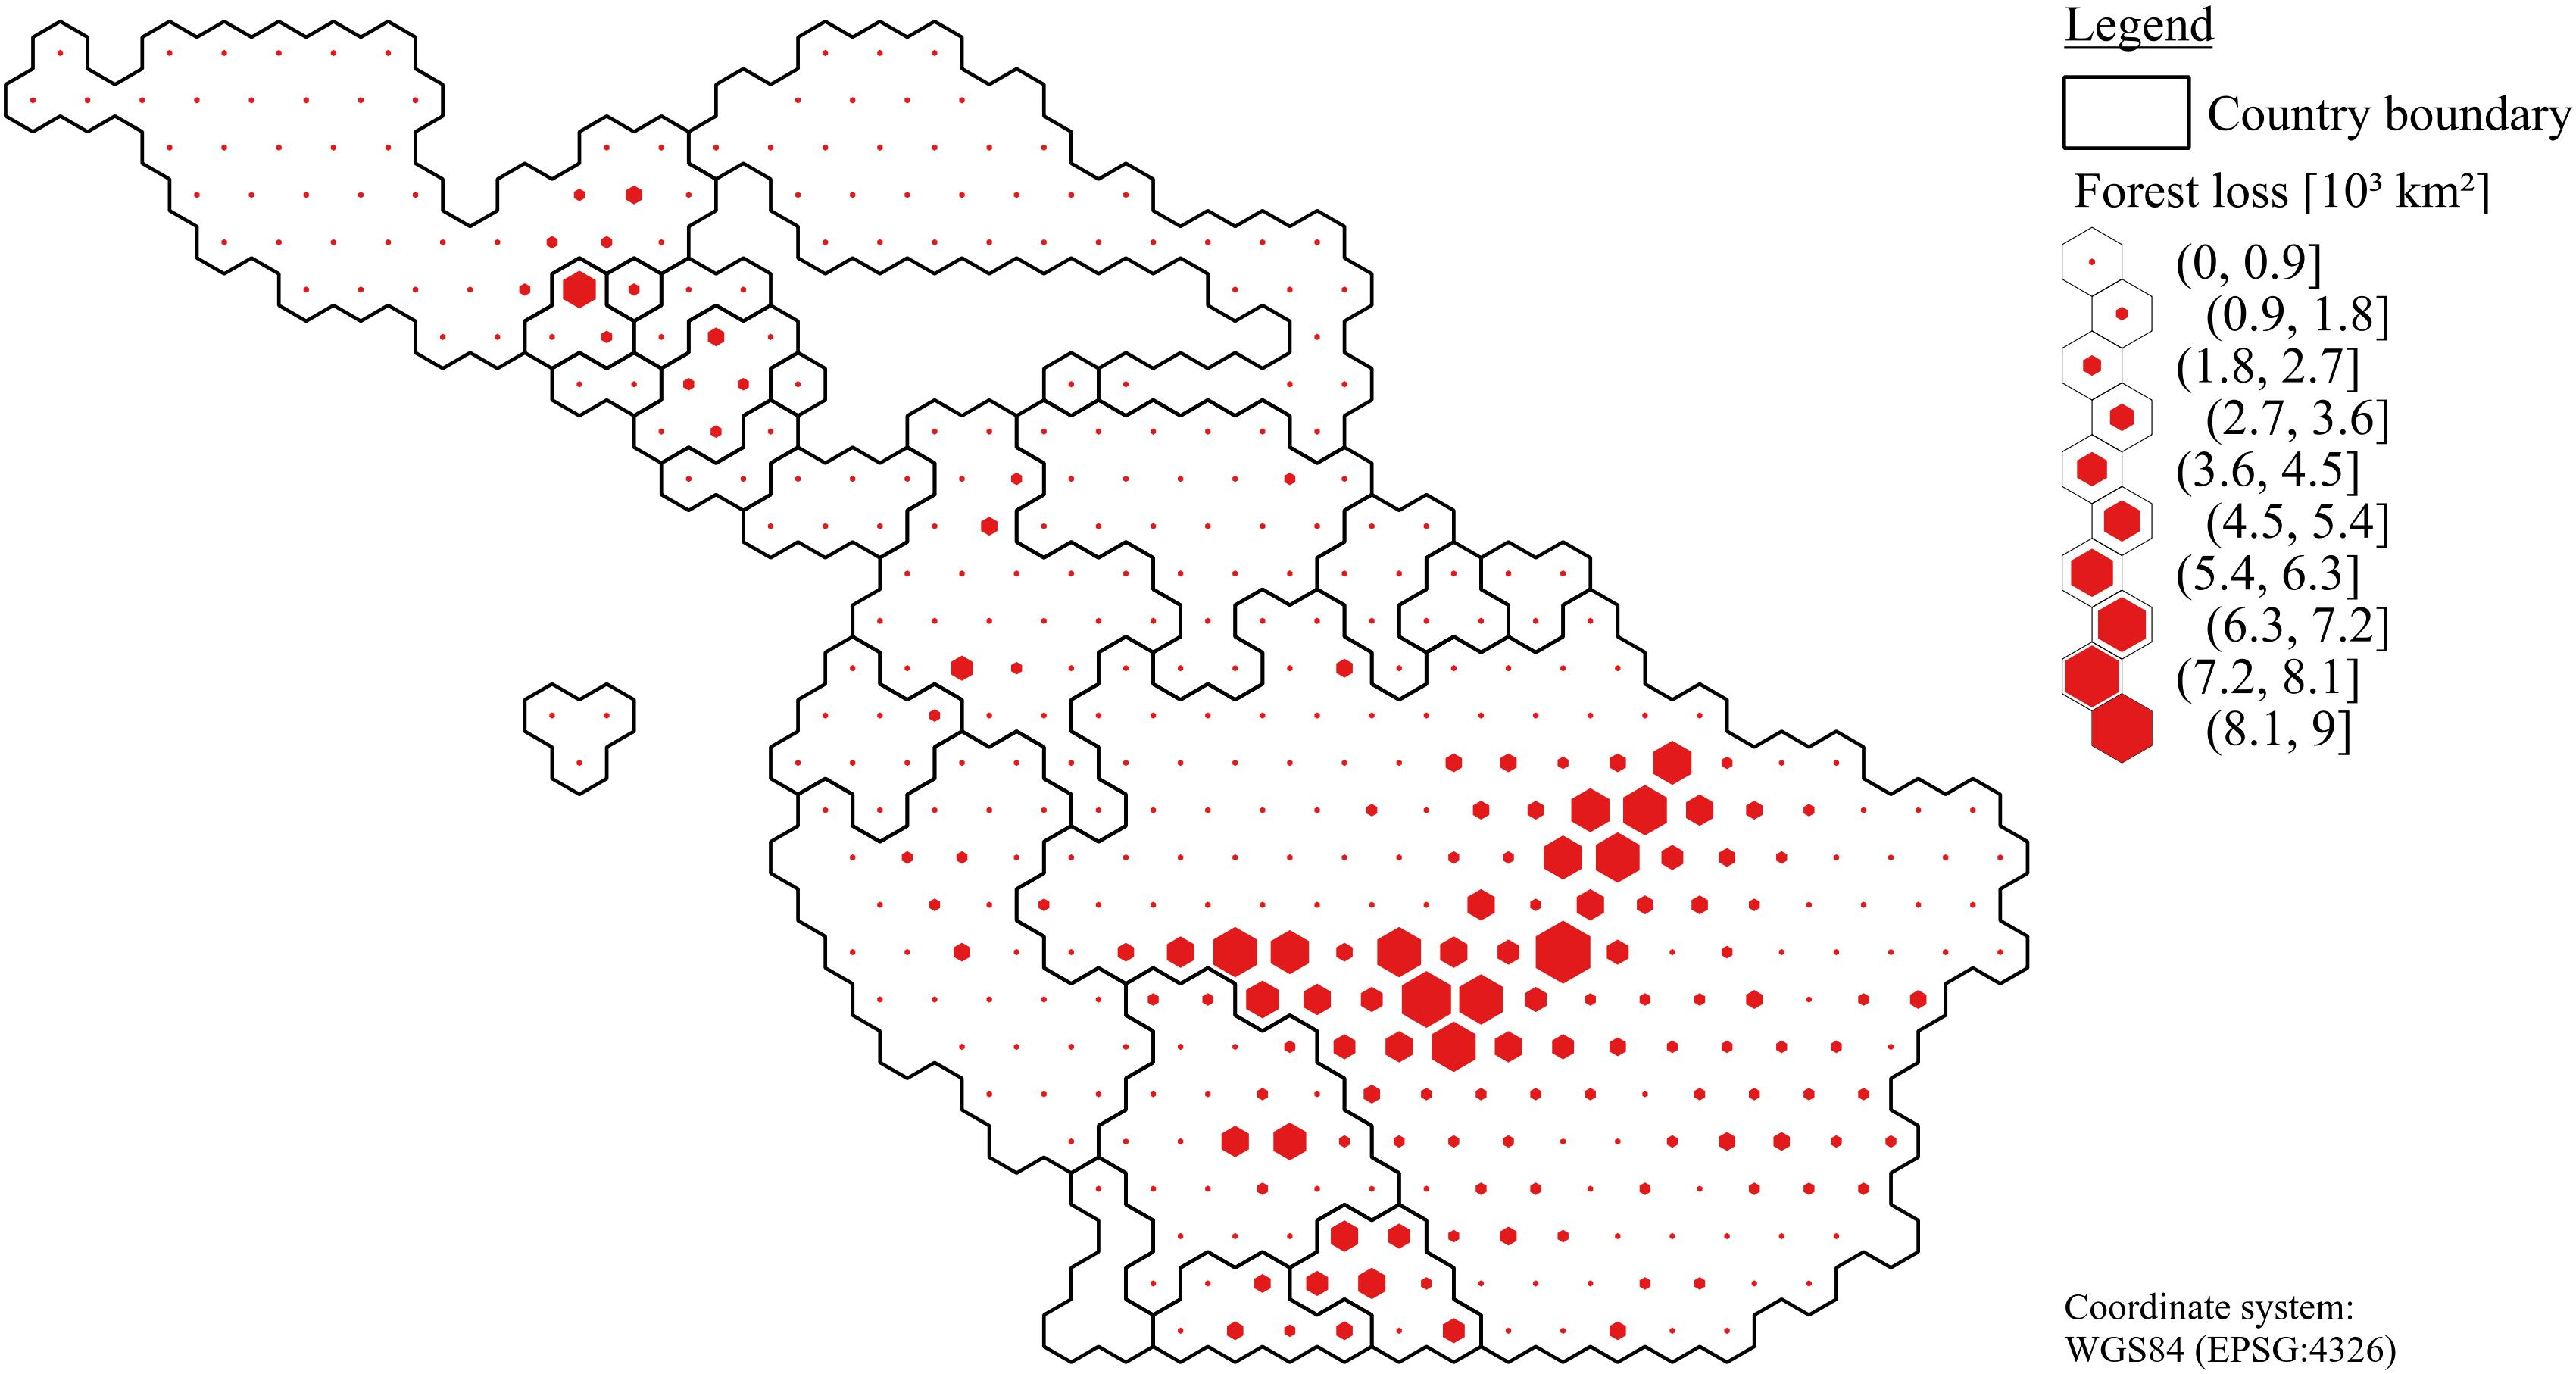
\includegraphics[scale=1]{img/americas_loss_frameless}
%				\caption[Ecosystem service values]{}
%				\label{fig:americasloss}
%			\end{figure}
%			\begin{figure}[ht]
%				\centering
%				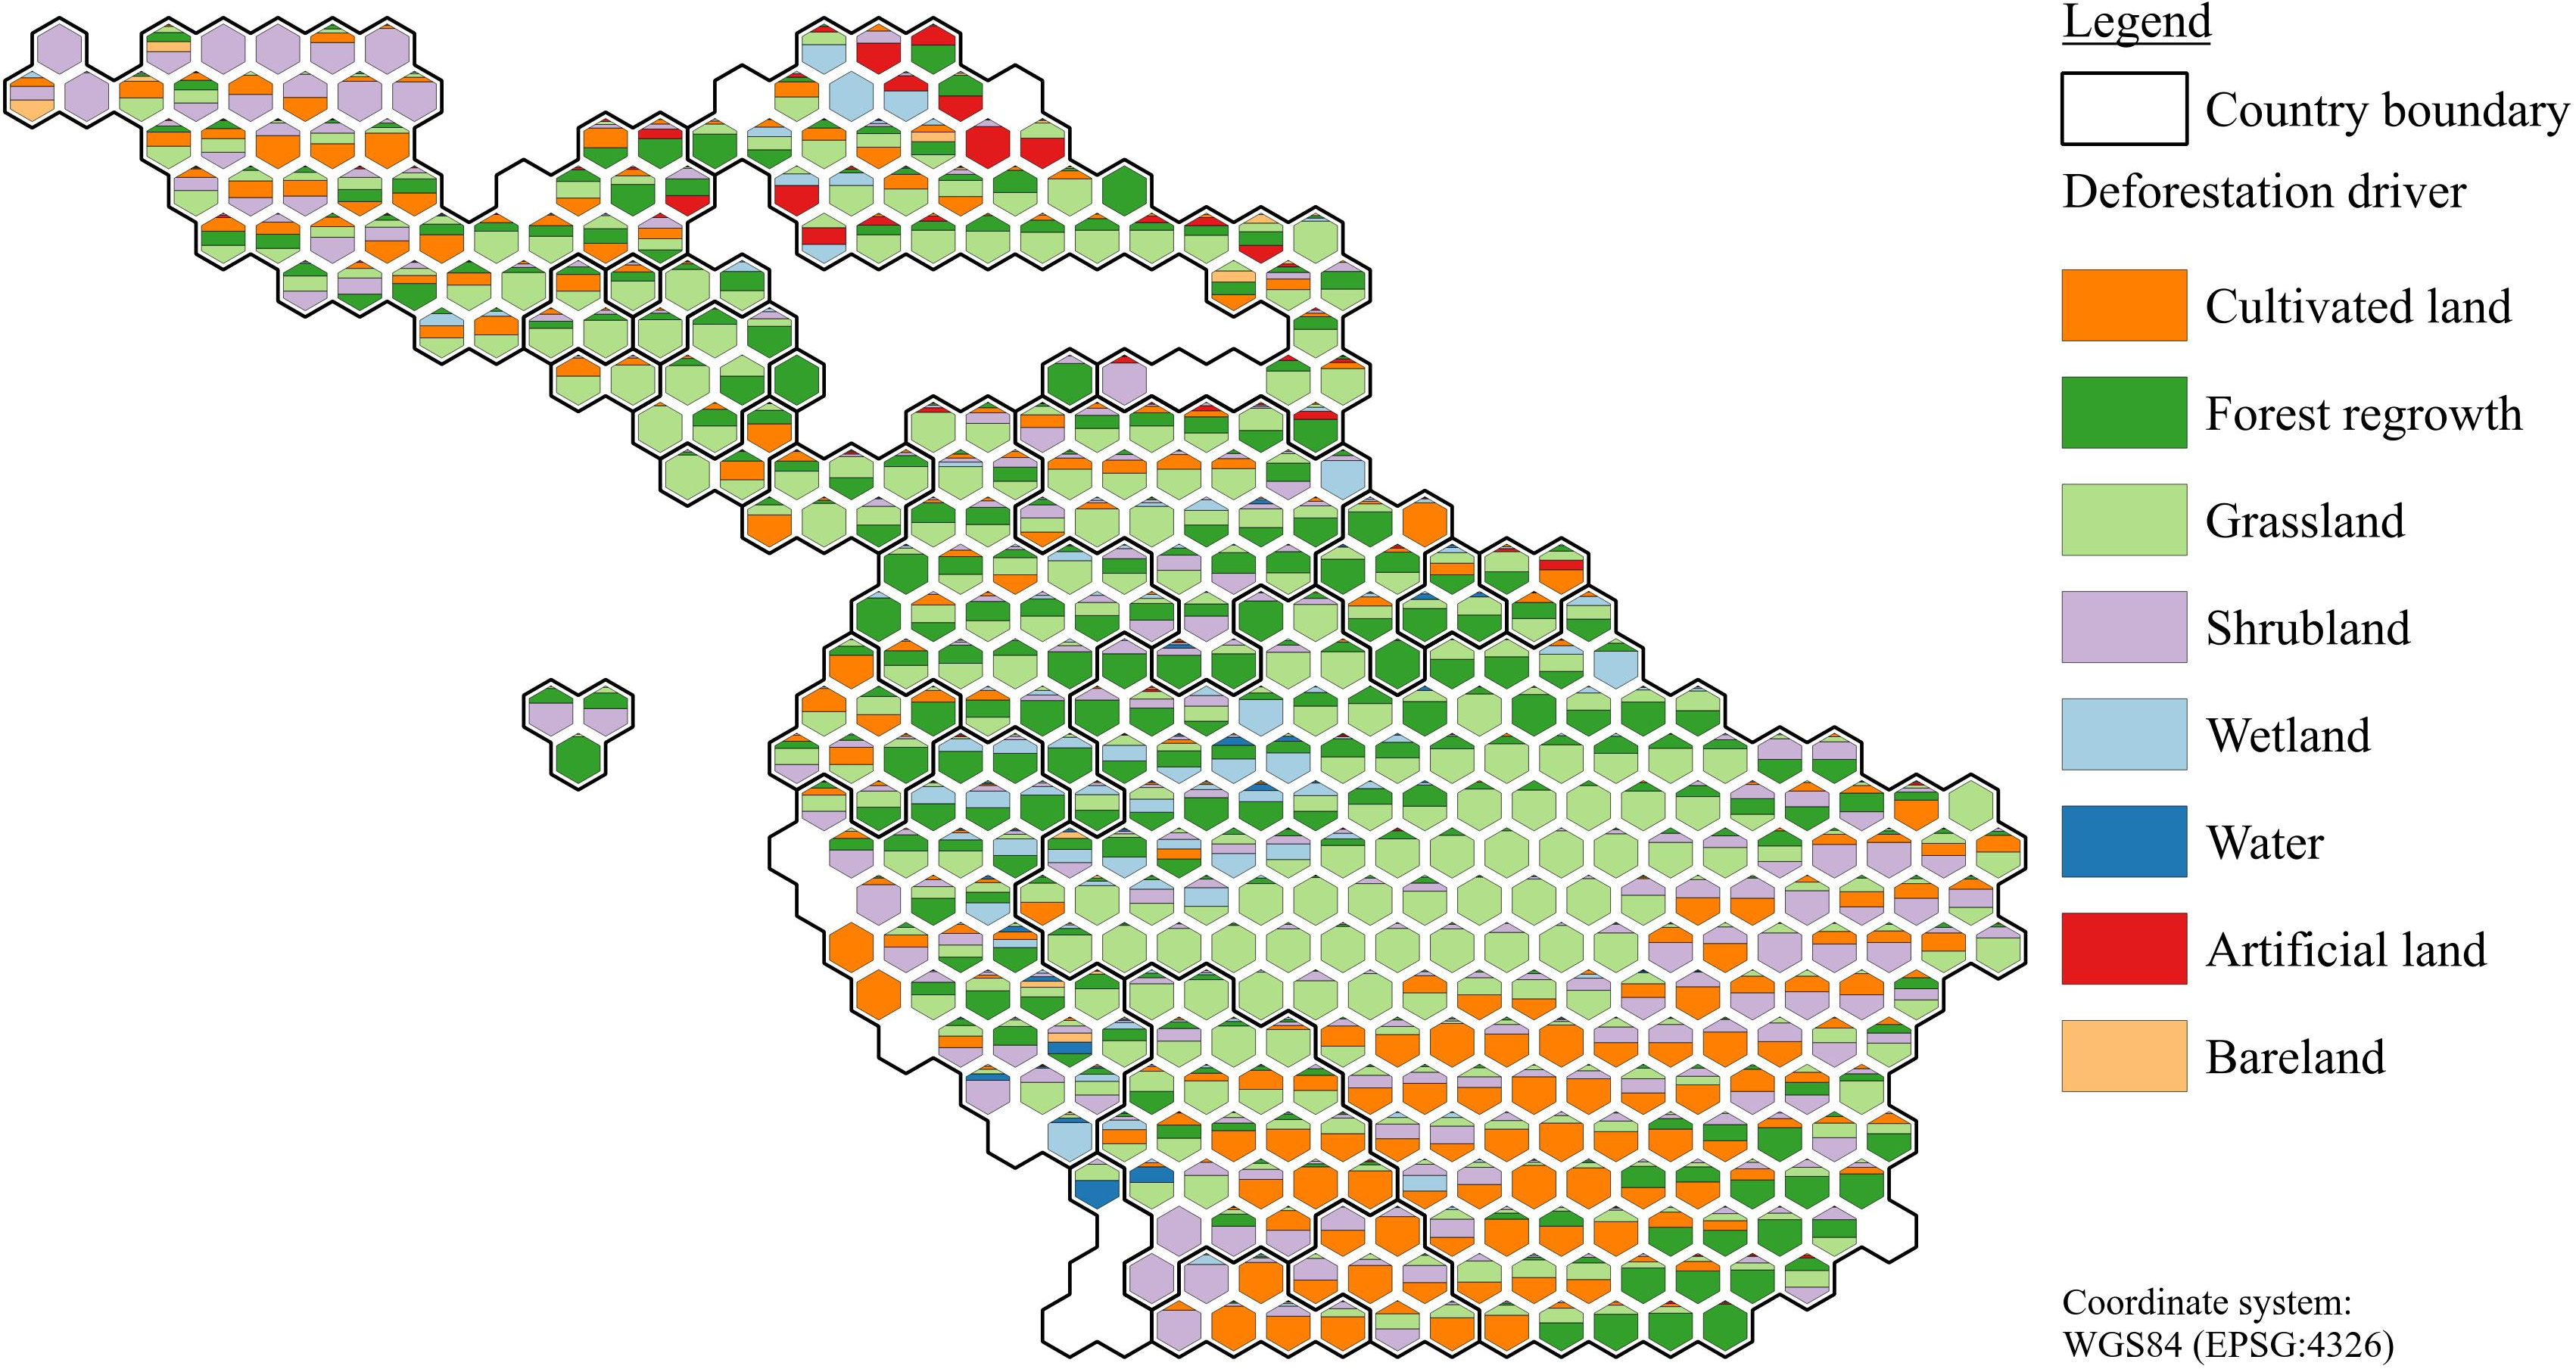
\includegraphics[scale=1]{img/americas_driver_frameless}
%				\caption[Ecosystem service values]{}
%				\label{fig:americasdriver}
%			\end{figure}

% ASIA
%			\begin{figure}[ht]
%				\centering
%				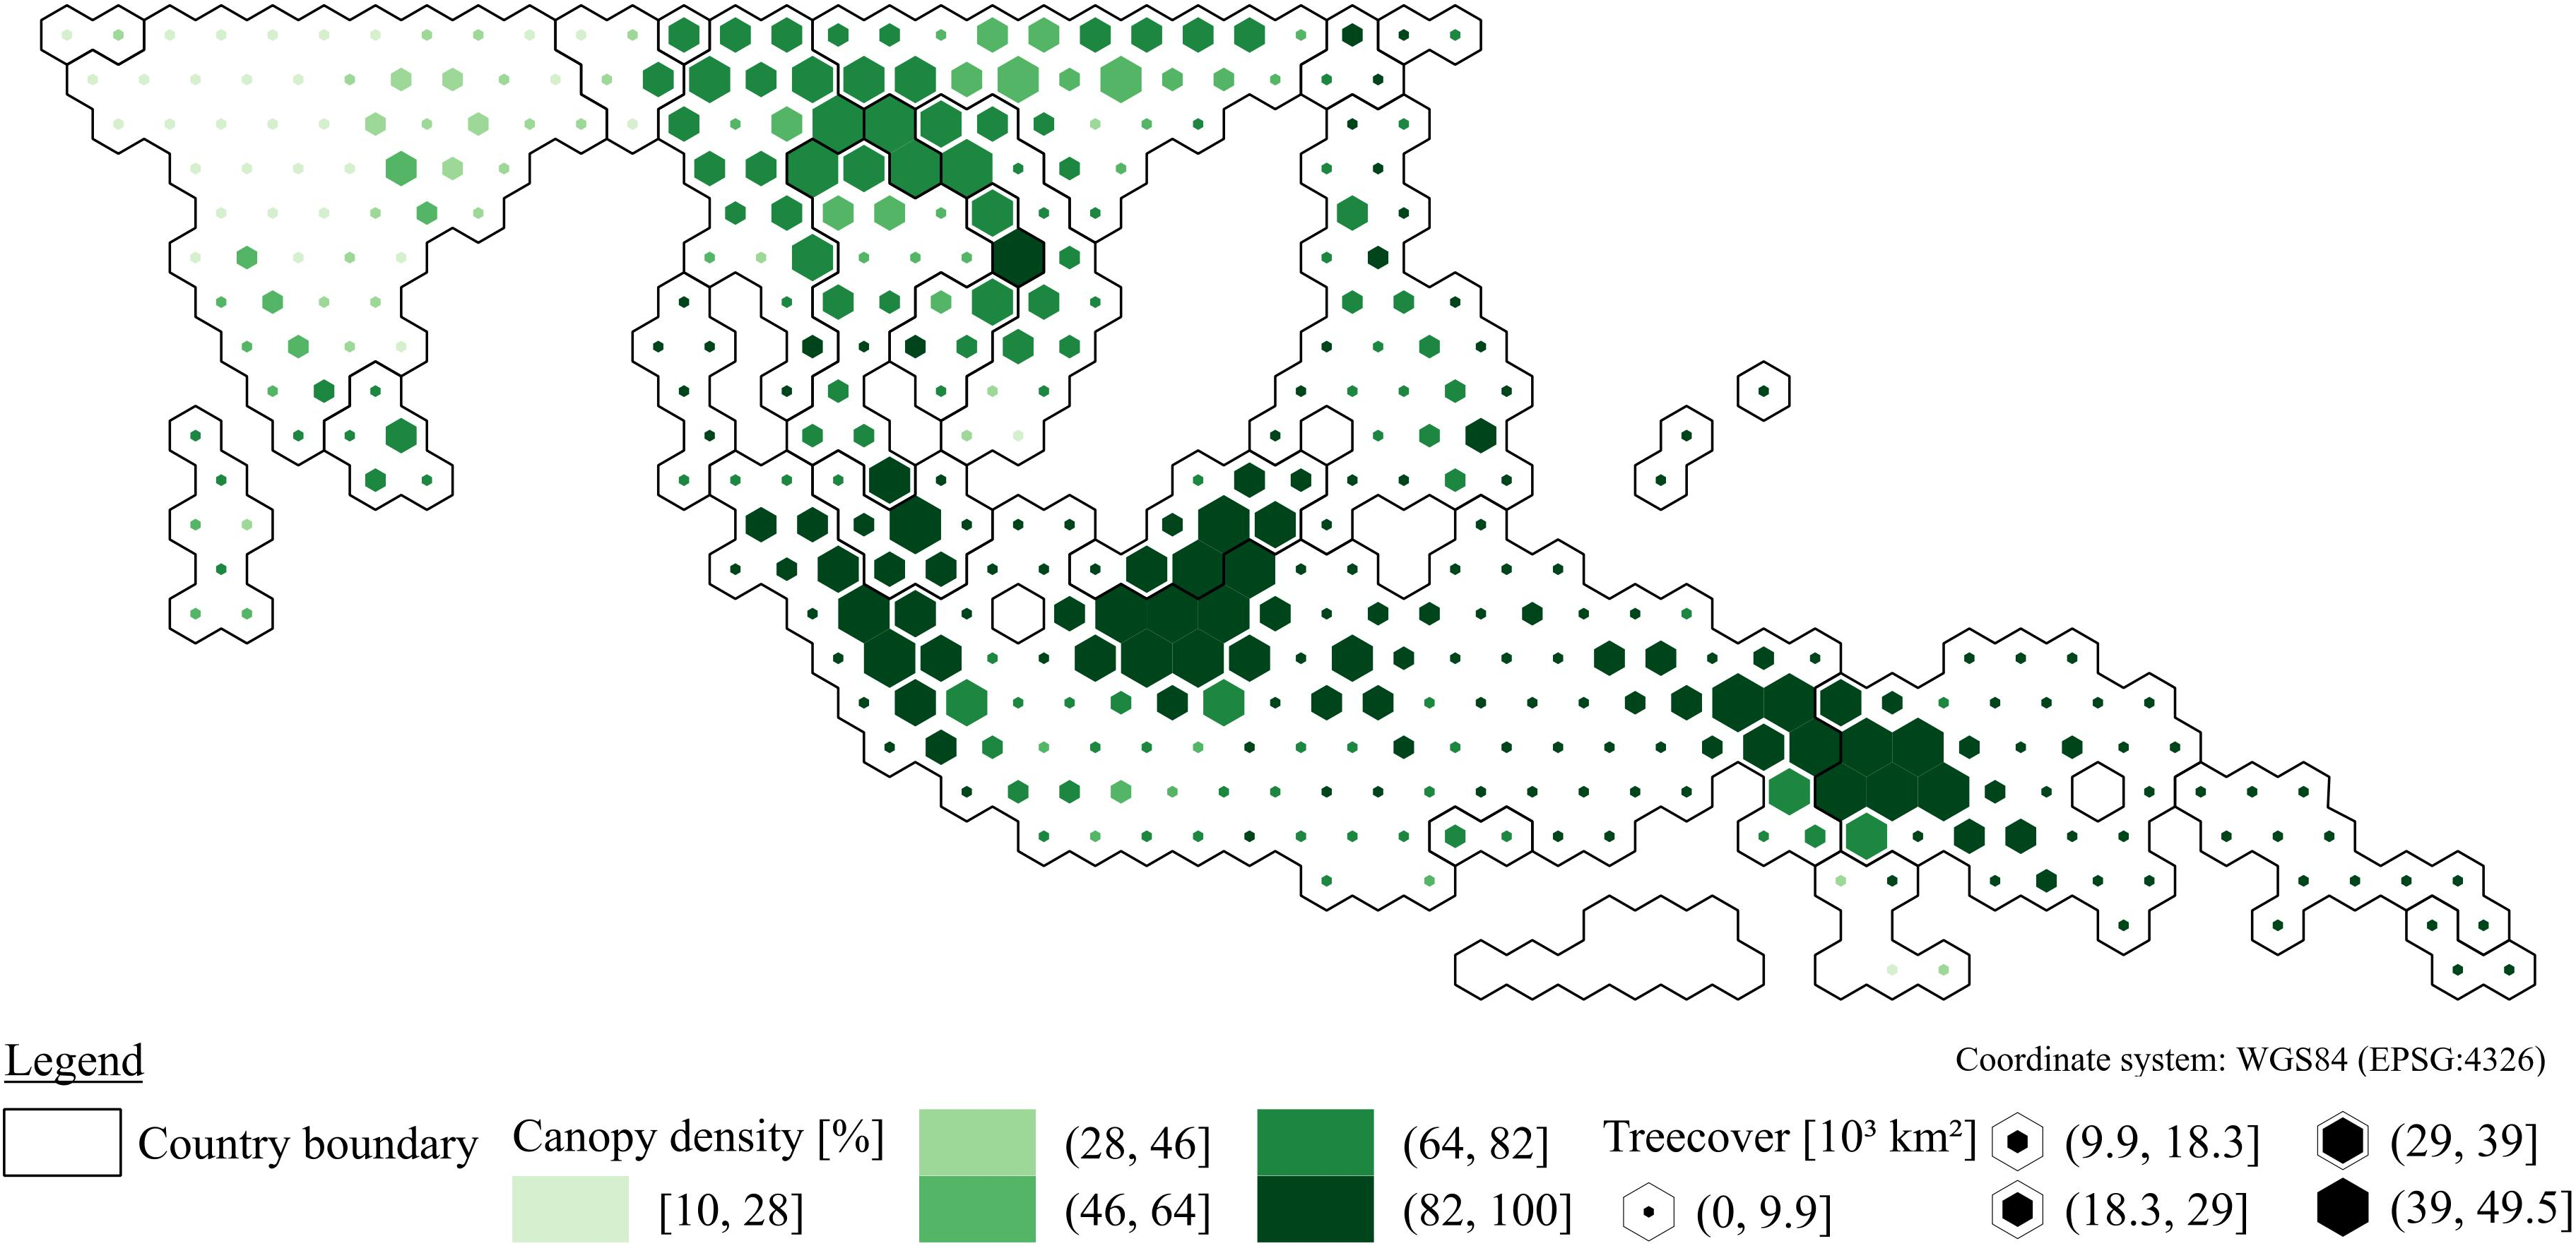
\includegraphics[scale=1]{img/asia_treecover_frameless}
%				\caption[Ecosystem service values]{}
%				\label{fig:asiacover}
%			\end{figure}
%			\begin{figure}[ht]
%				\centering
%				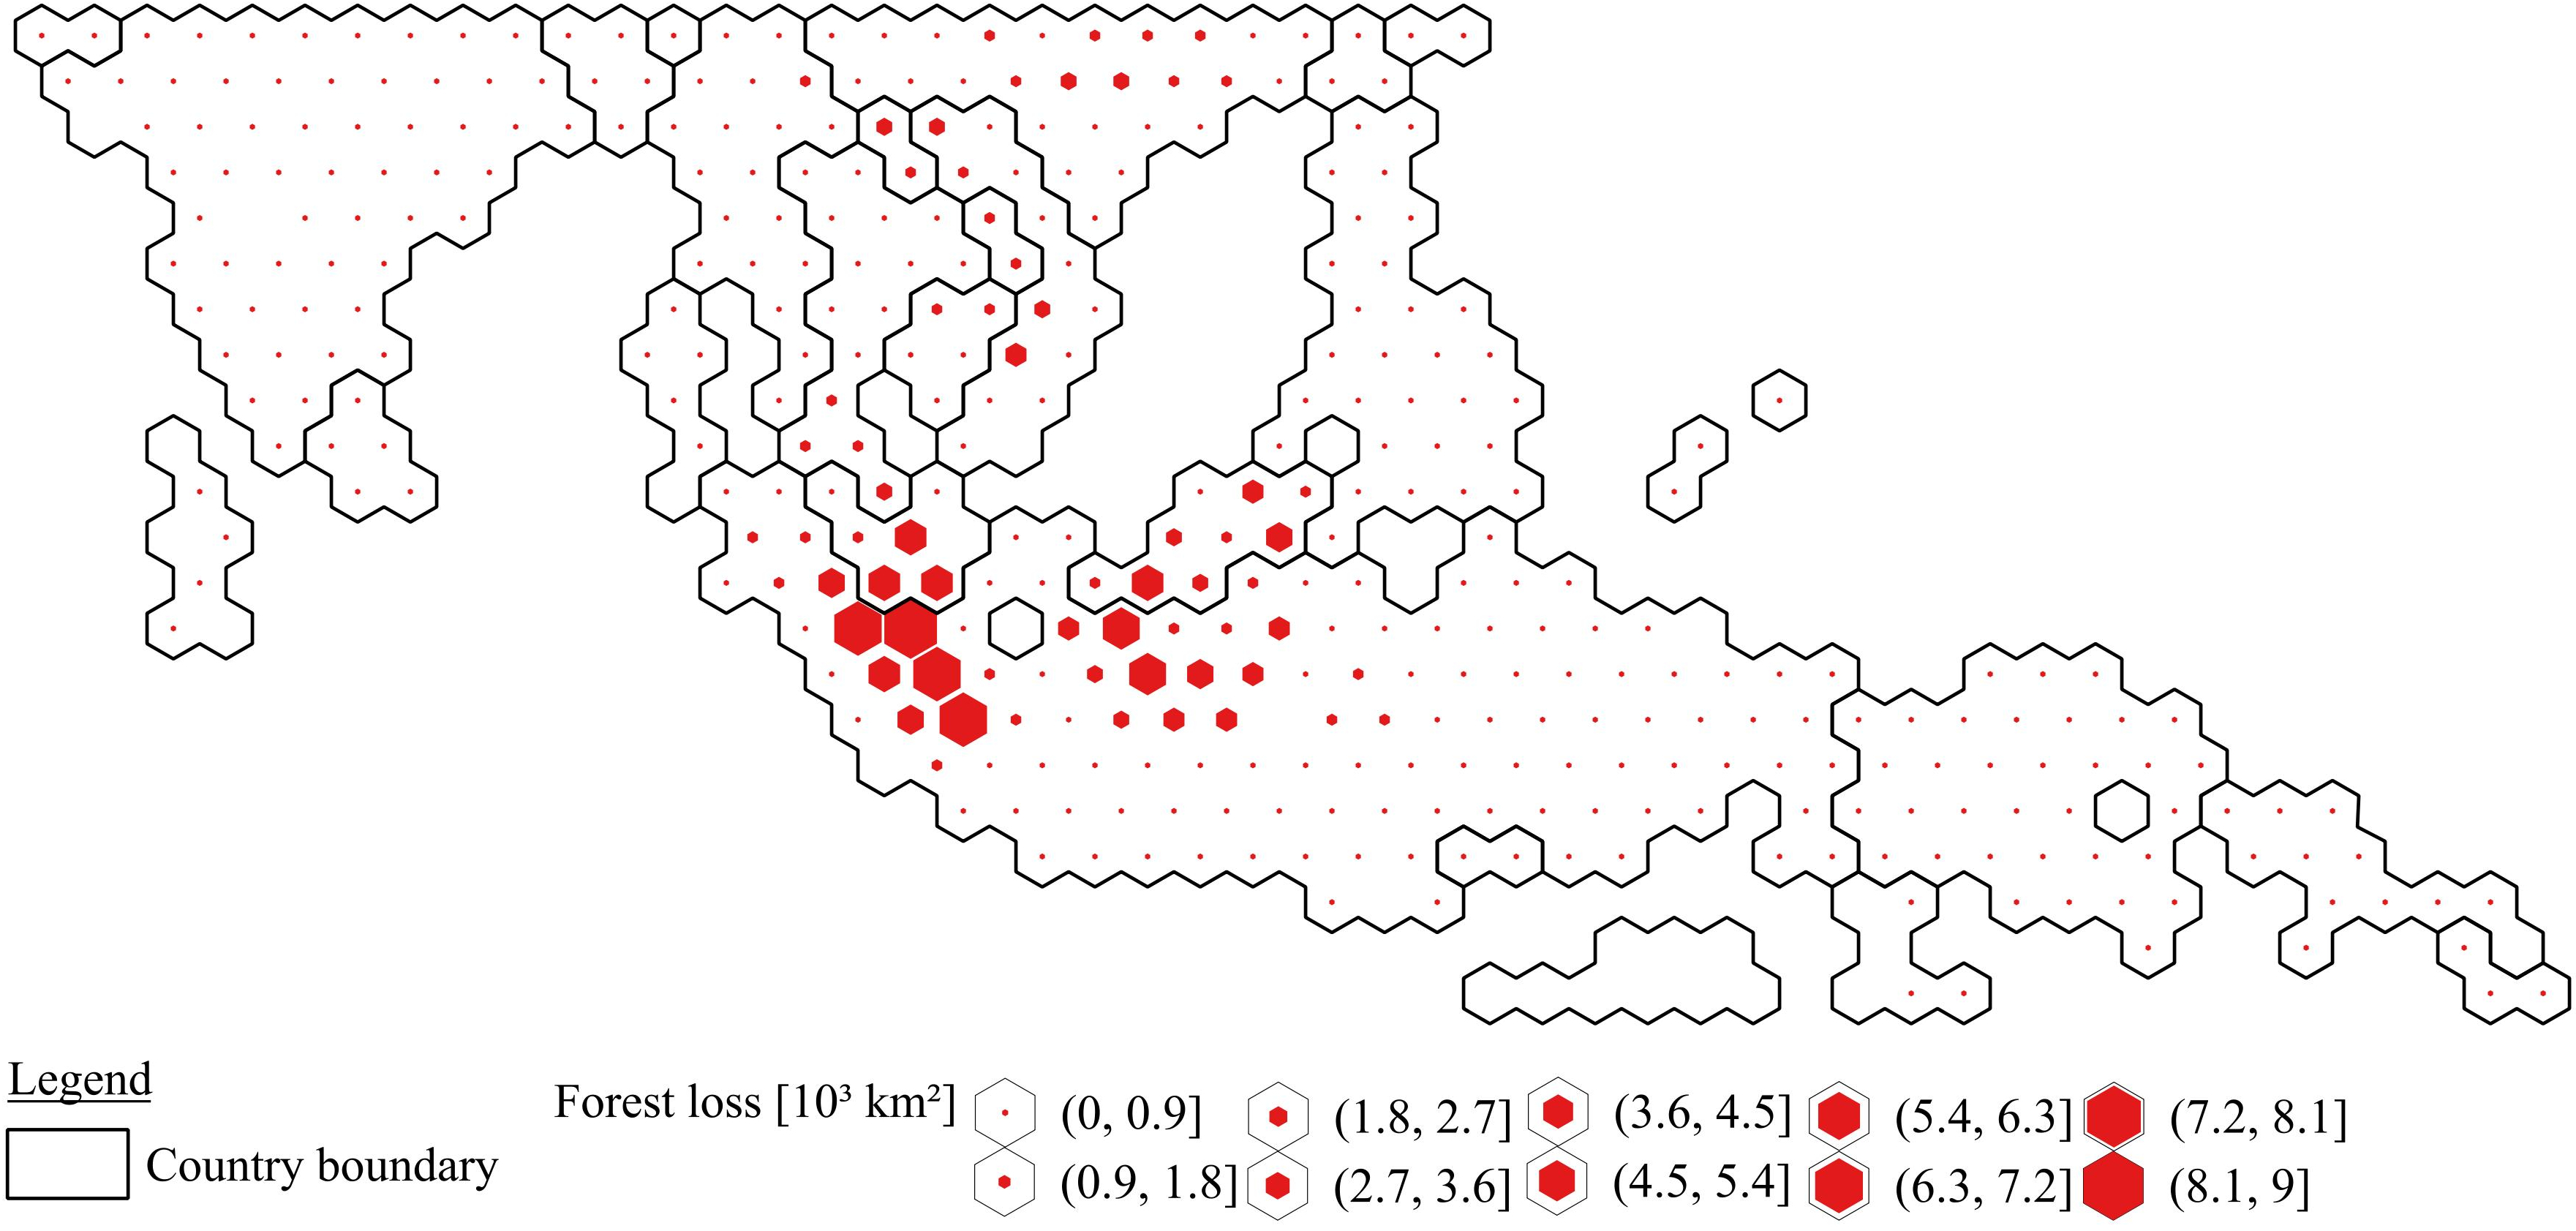
\includegraphics[scale=1]{img/asia_loss_frameless}
%				\caption[Ecosystem service values]{}
%				\label{fig:asialoss}
%			\end{figure}
%			\begin{figure}[ht]
%				\centering
%				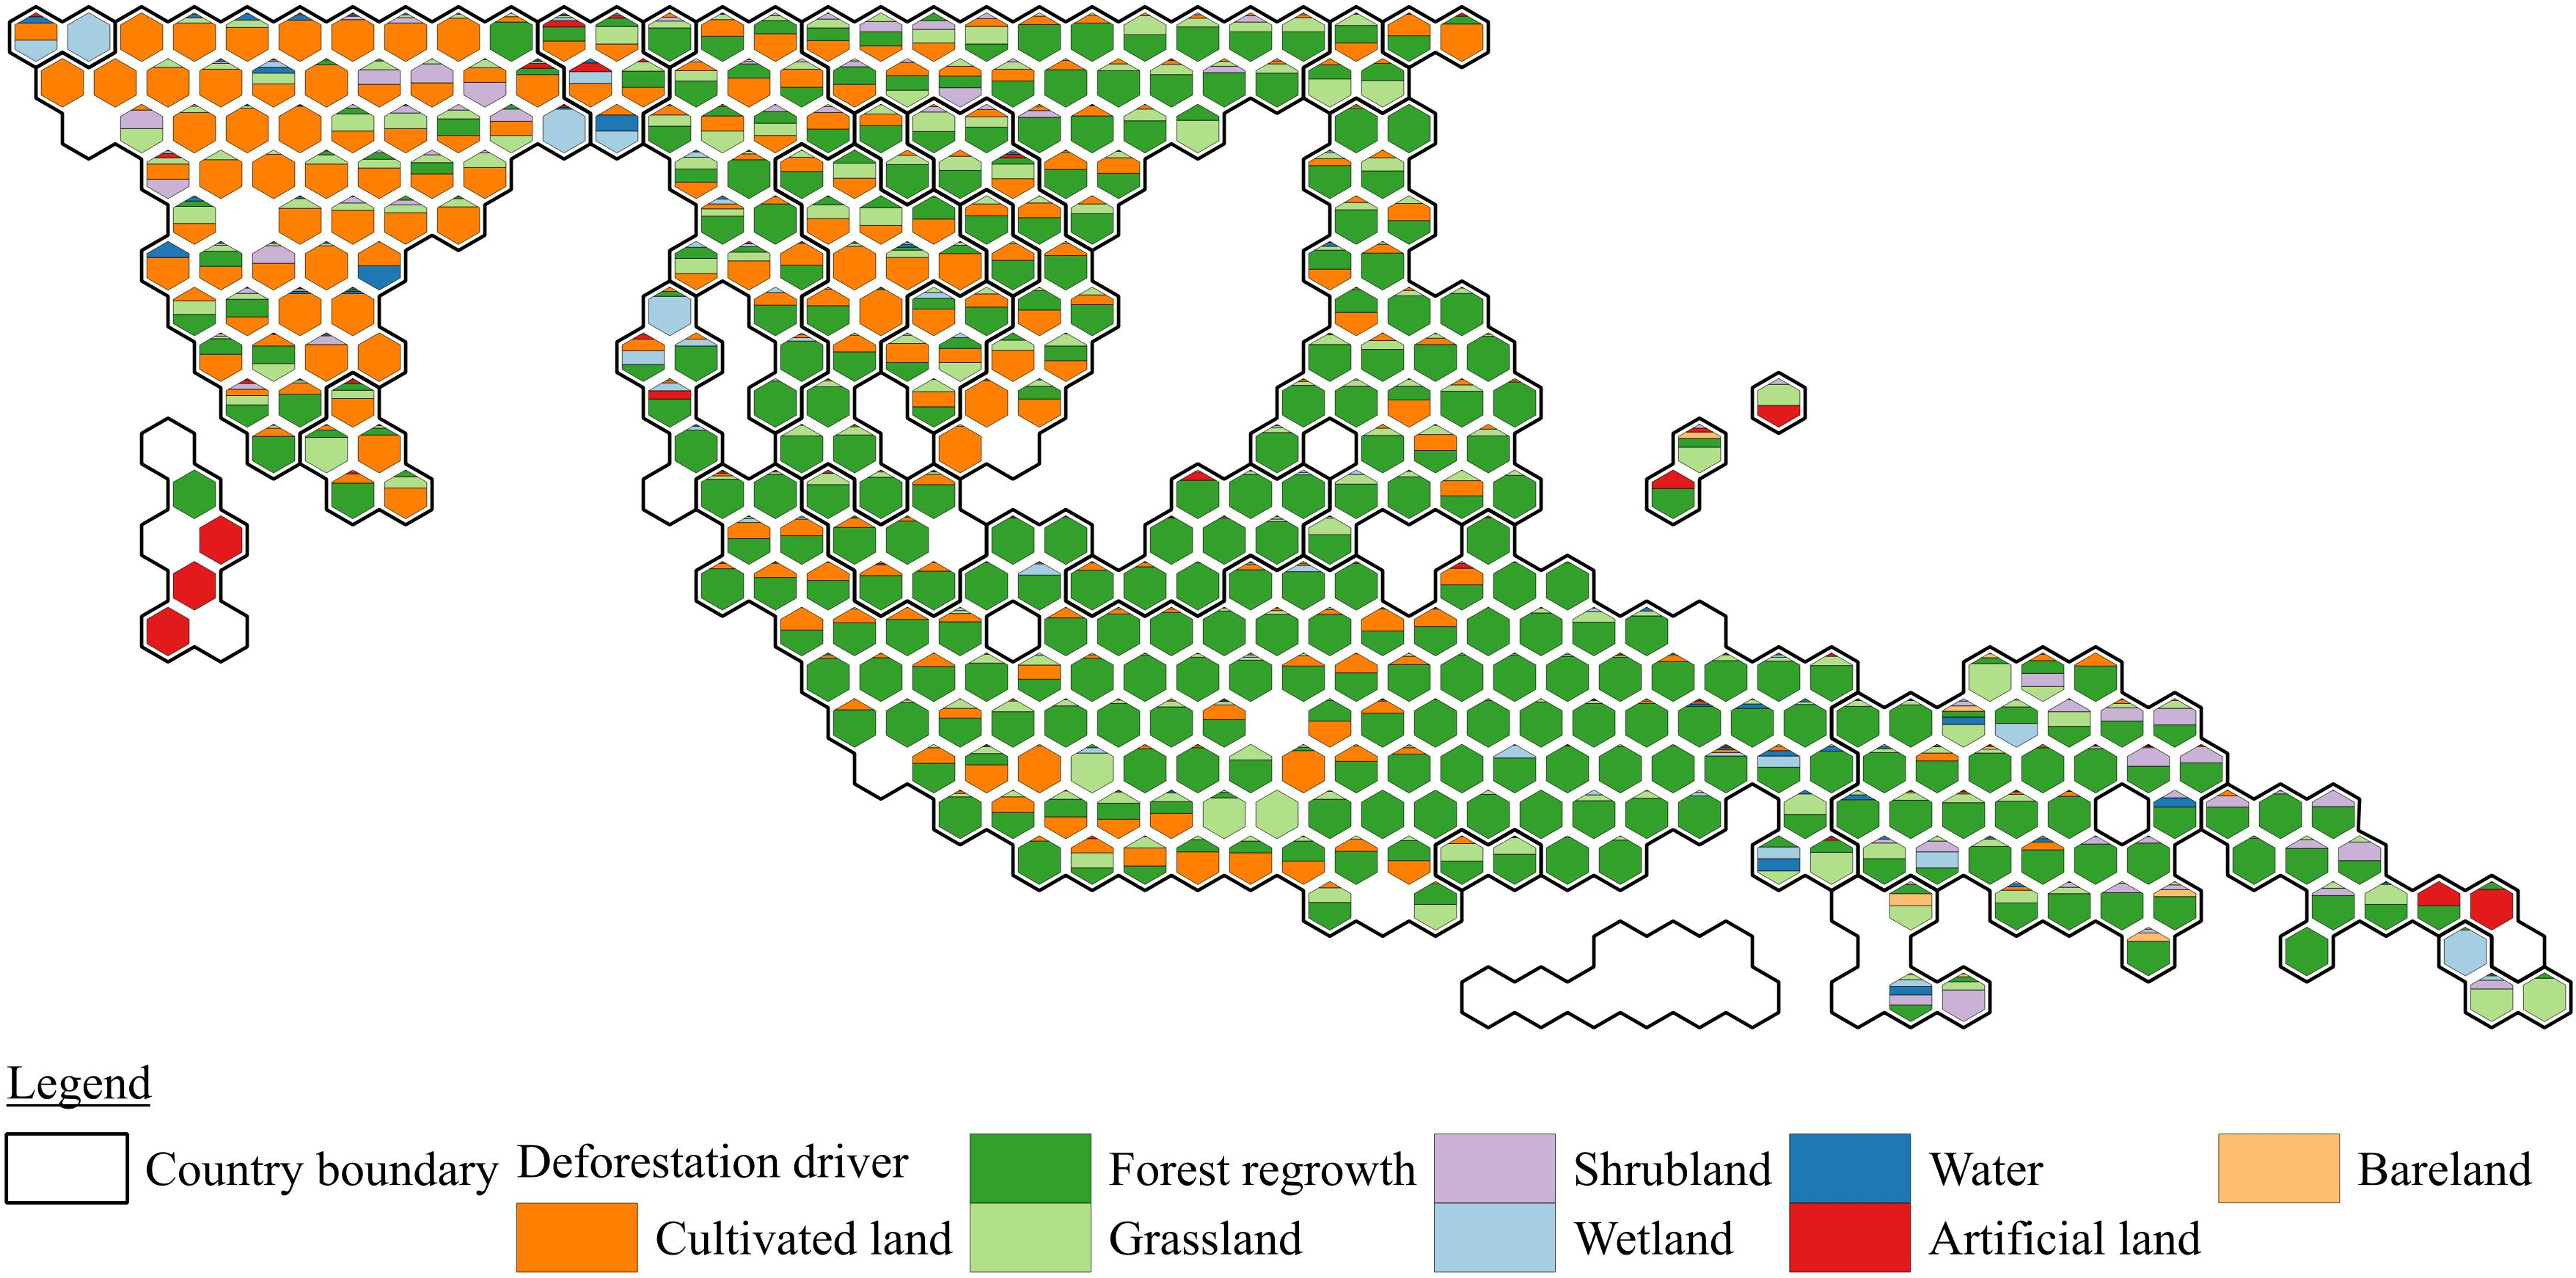
\includegraphics[scale=1]{img/asia_driver_frameless}
%				\caption[Ecosystem service values]{}
%				\label{fig:asiadriver}
%			\end{figure}

% AFRICA
%			\begin{figure}[ht]
%				\centering
%				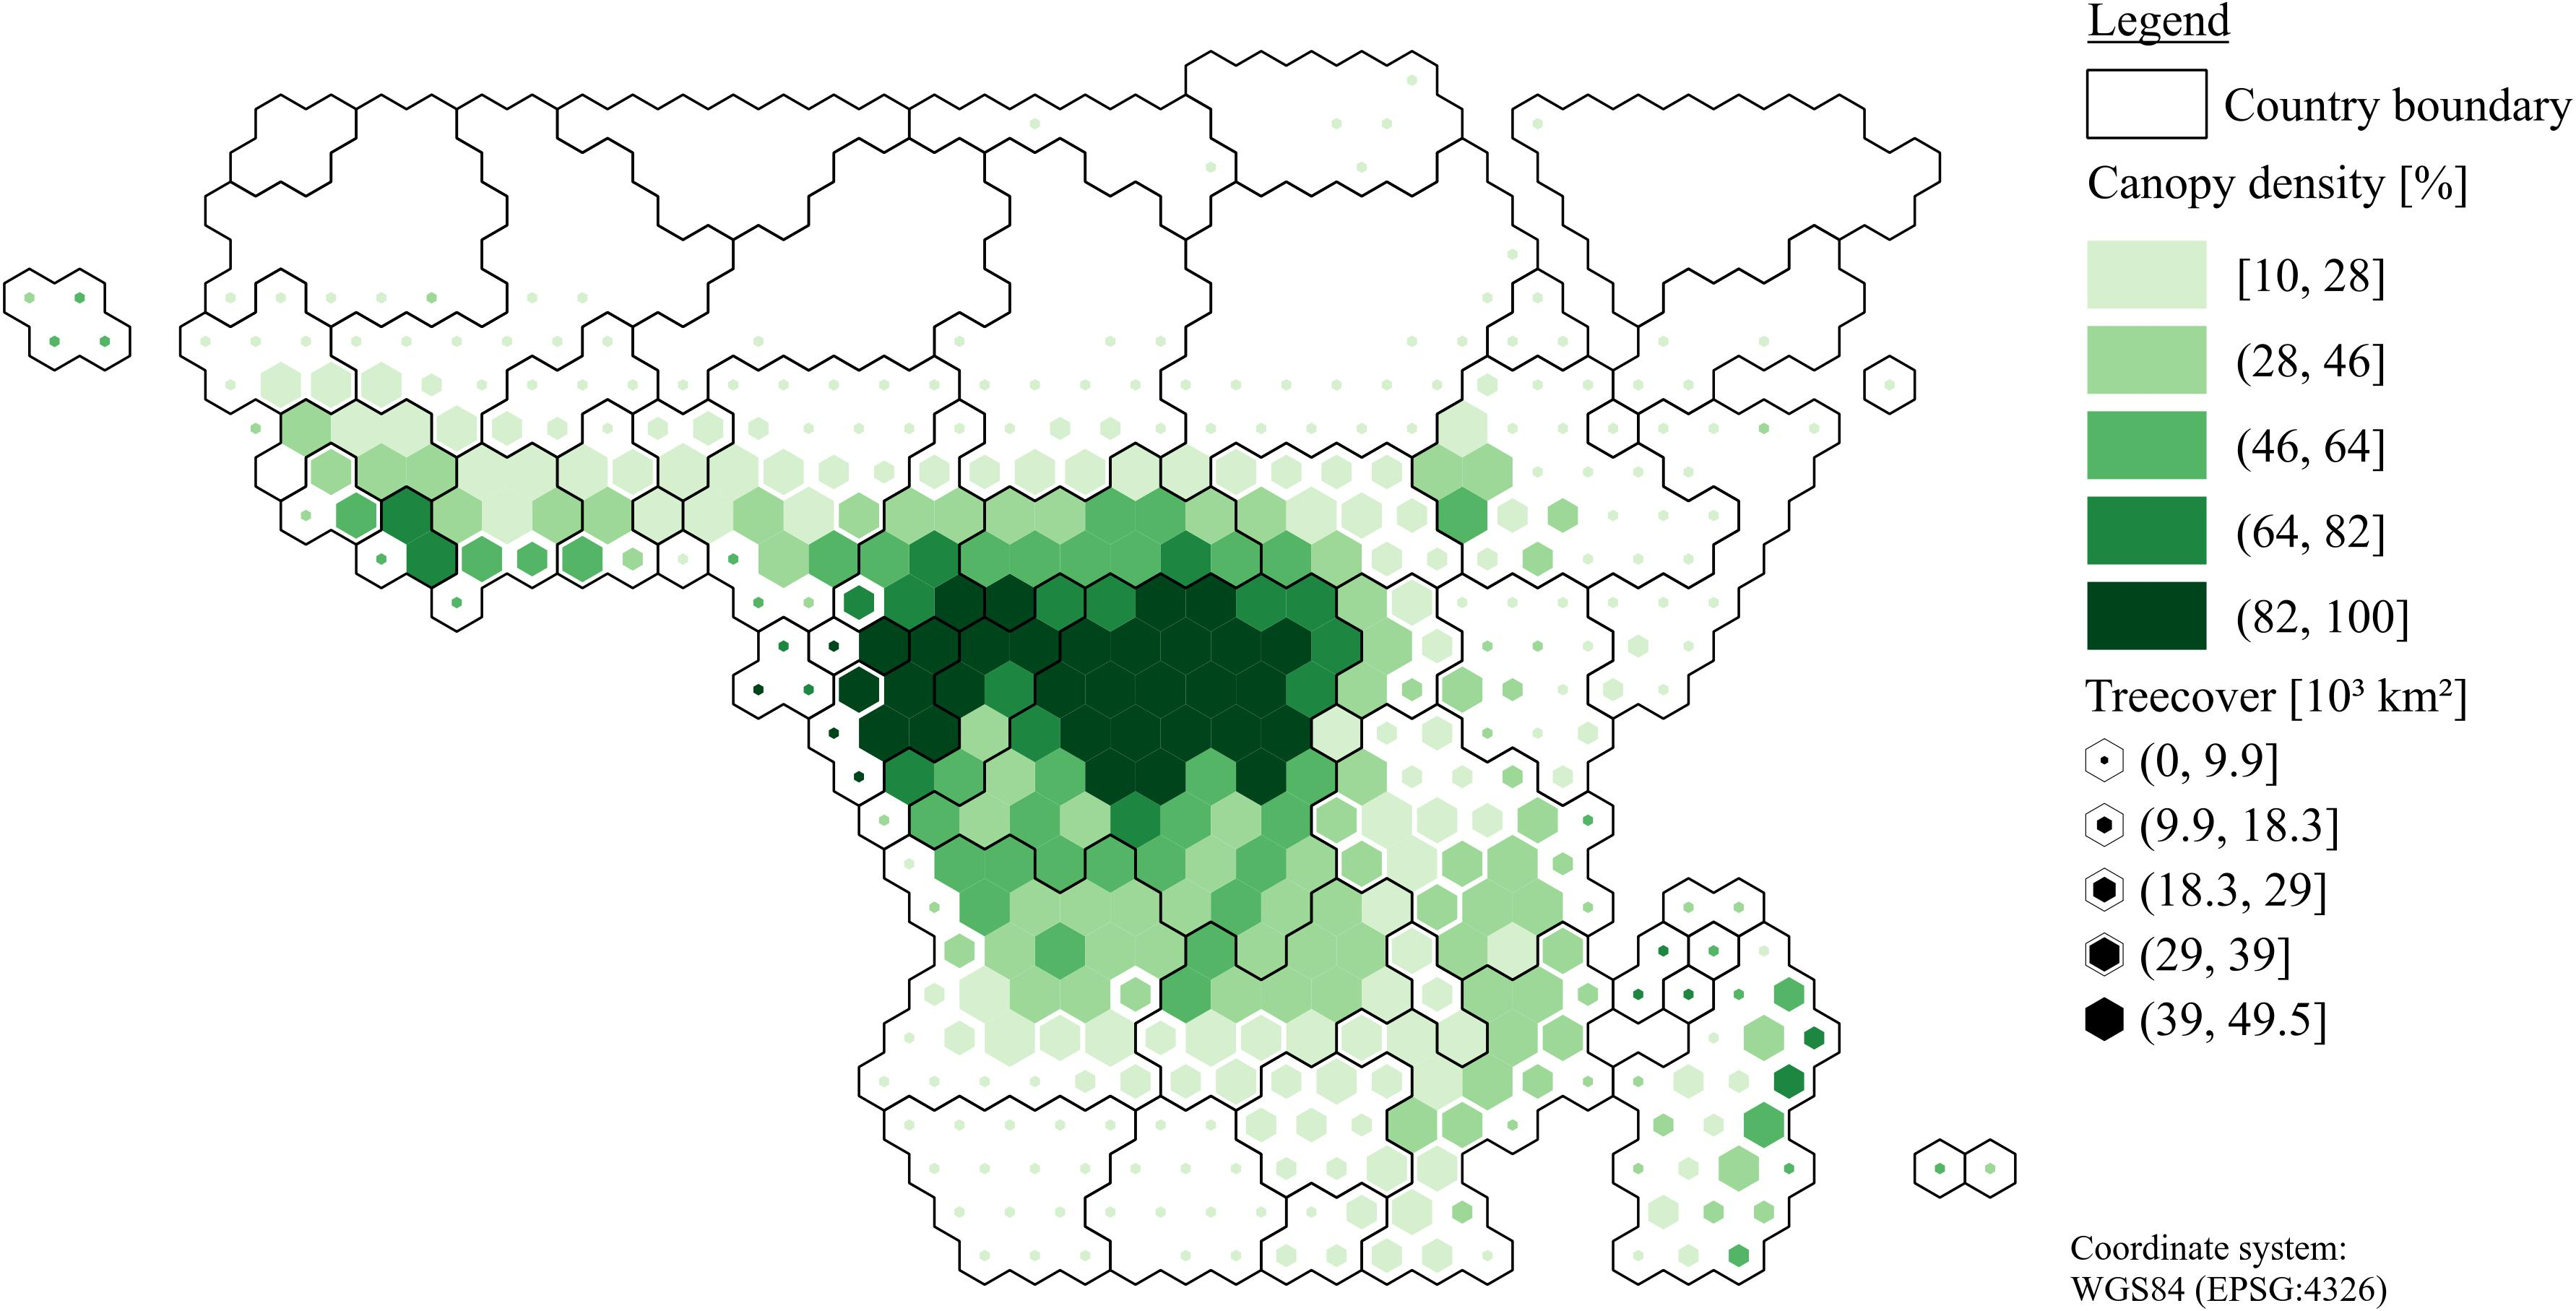
\includegraphics[scale=1]{img/africa_treecover_frameless}
%				\caption[Ecosystem service values]{}
%				\label{fig:africacover}
%			\end{figure}
%			\begin{figure}[ht]
%				\centering
%				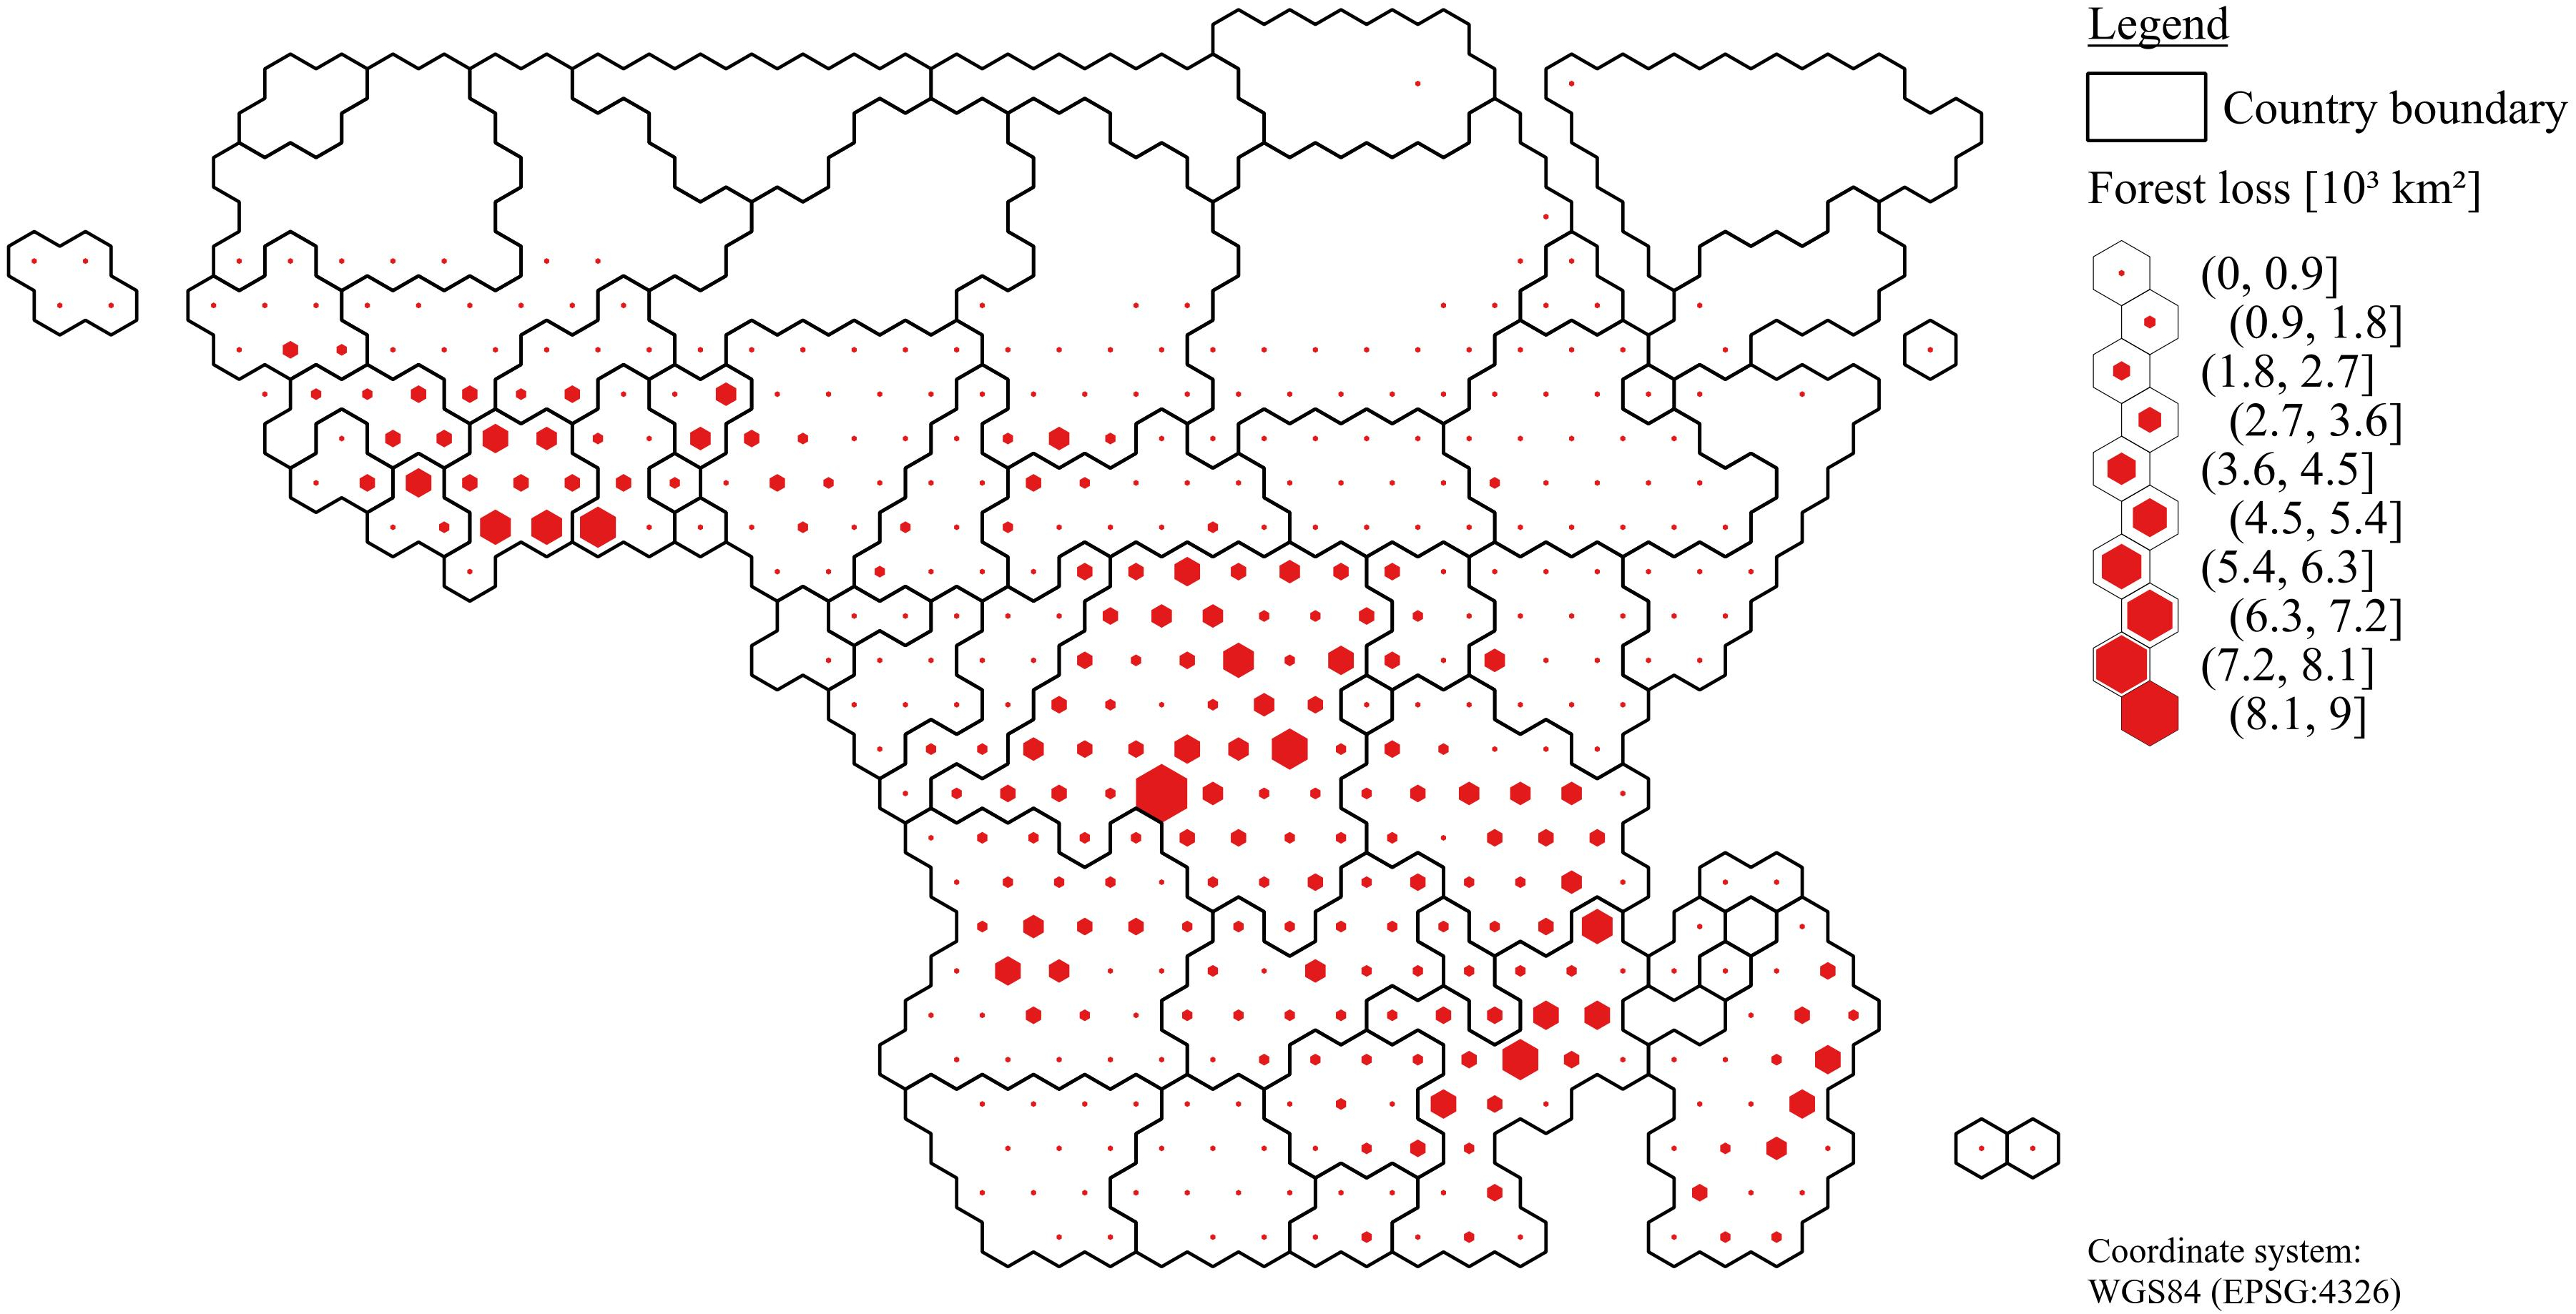
\includegraphics[scale=1]{img/africa_loss_frameless}
%				\caption[Ecosystem service values]{}
%				\label{fig:africaloss}
%			\end{figure}
%			\begin{figure}[ht]
%				\centering
%				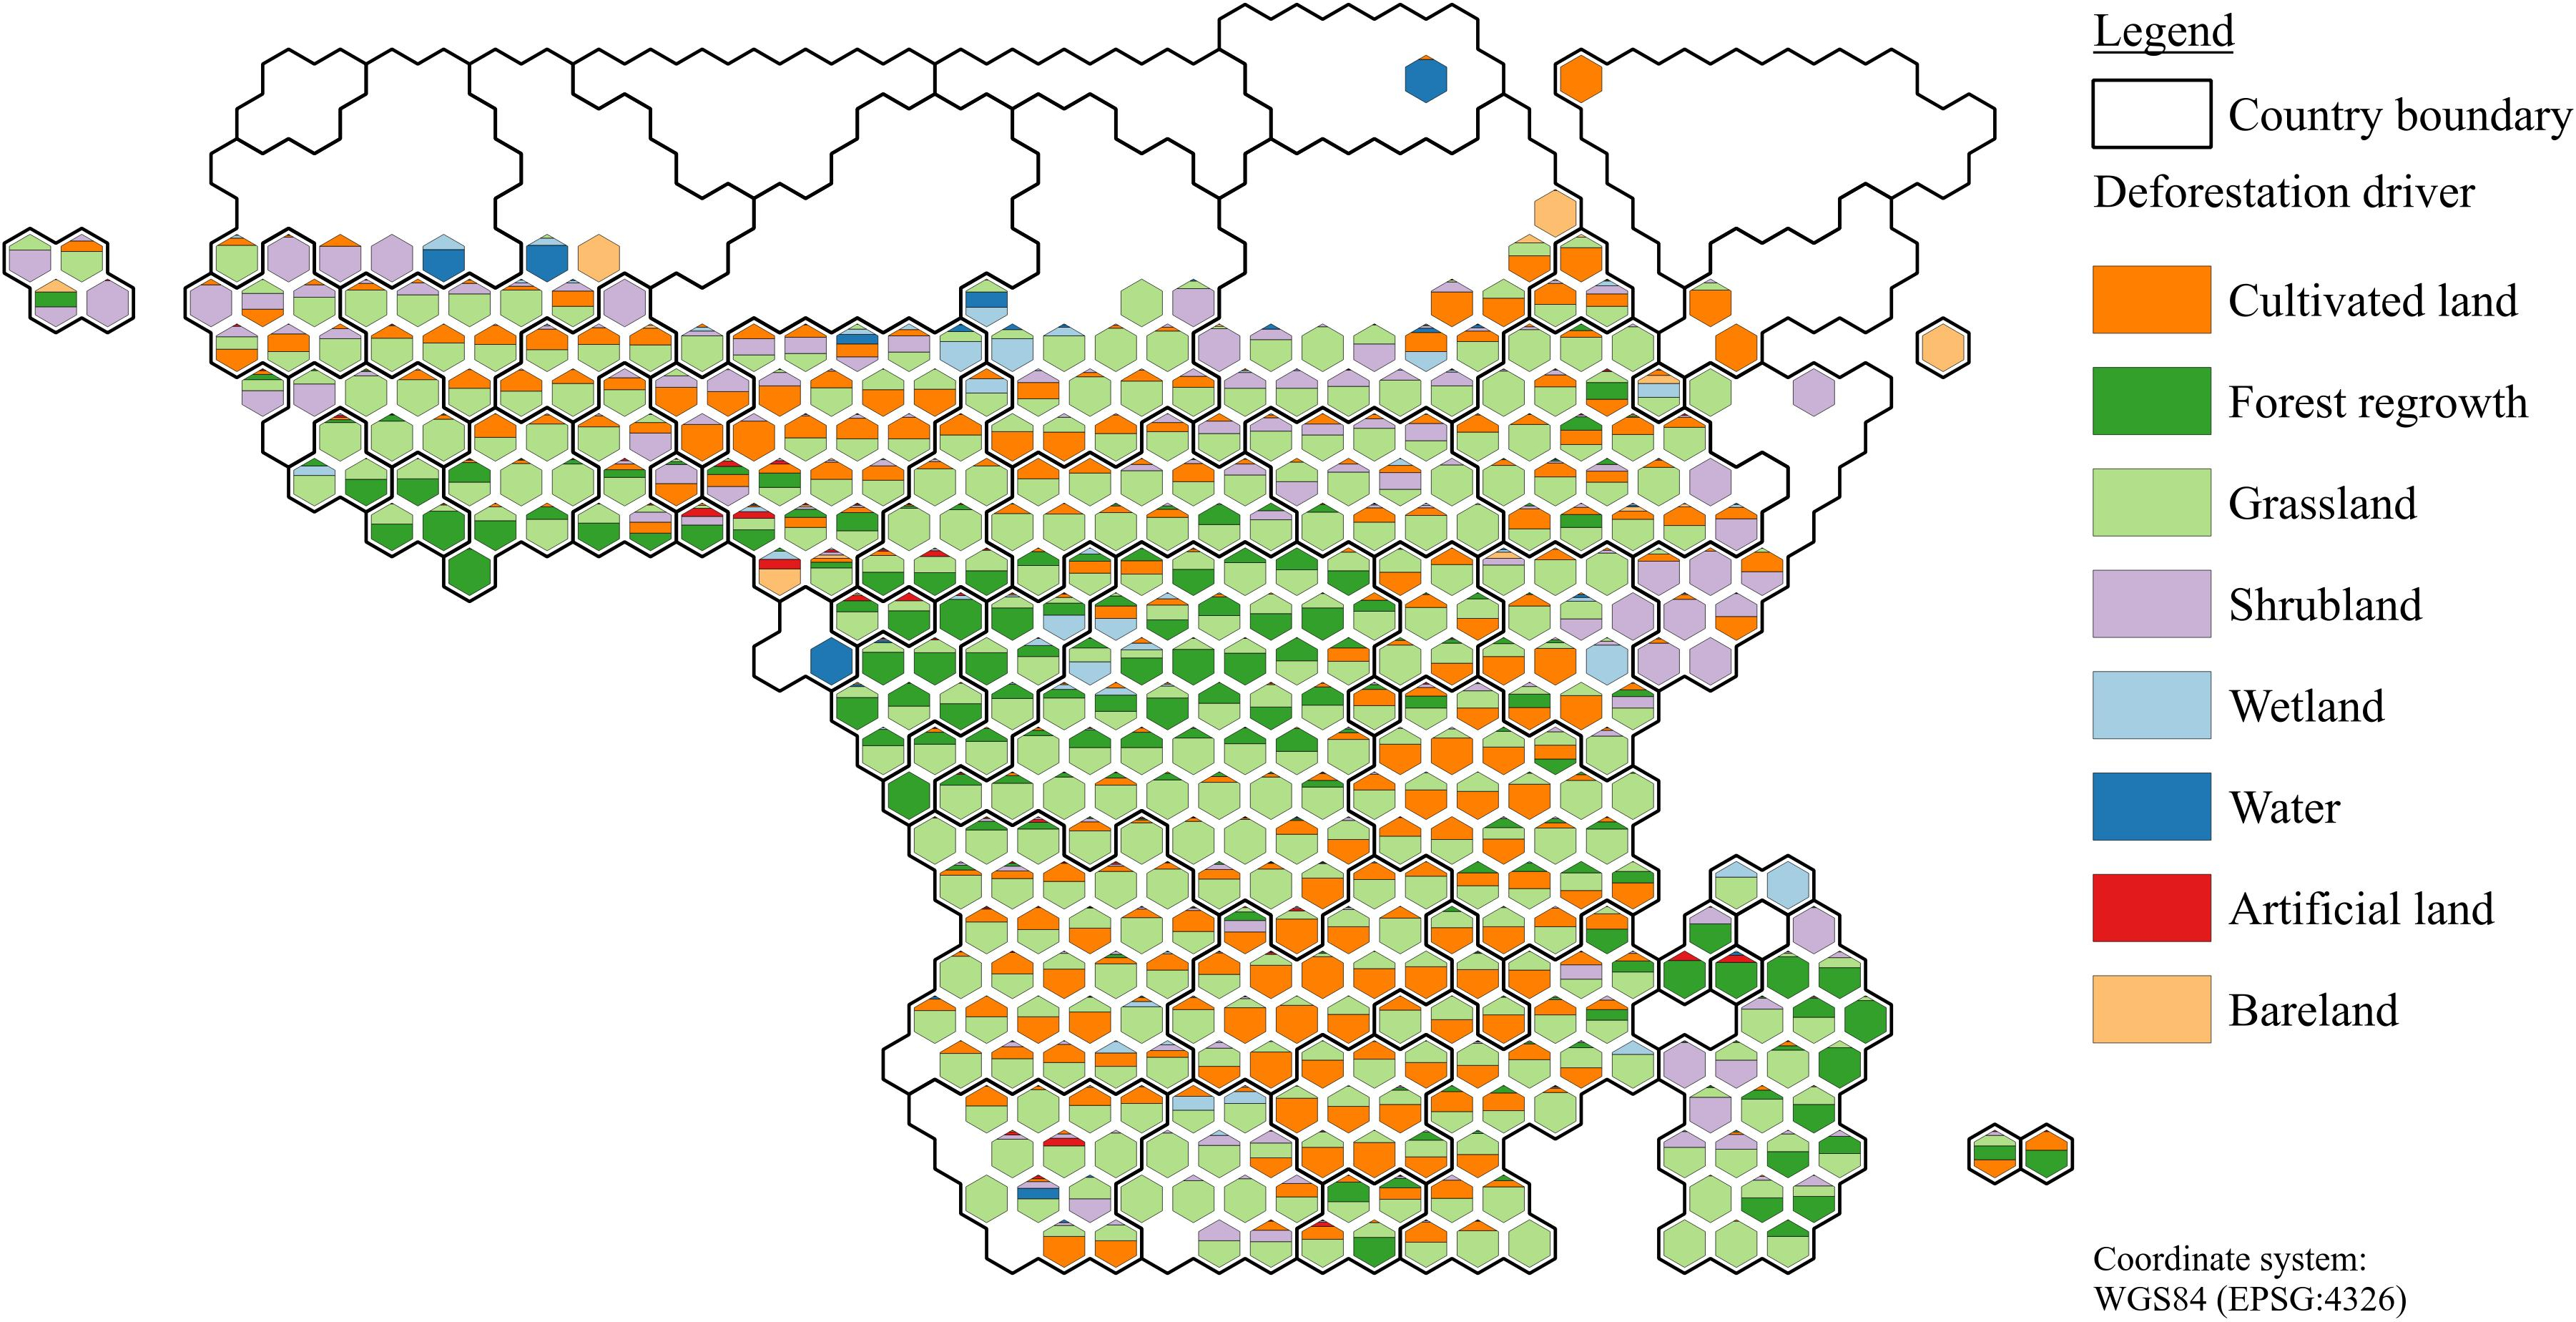
\includegraphics[scale=1]{img/africa_driver_frameless}
%				\caption[Ecosystem service values]{}
%				\label{fig:africadriver}
%			\end{figure}


% EMISSIONS
%		\begin{figure}[ht]
%			\centering
%			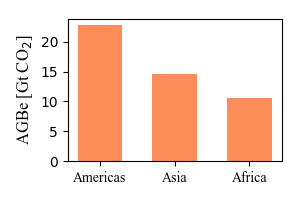
\includegraphics[scale=1]{img/agbe}
%			\caption[Ecosystem service values]{}
%			\label{fig:agbe}
%		\end{figure}
%		\begin{figure}[ht]
%			\centering
%			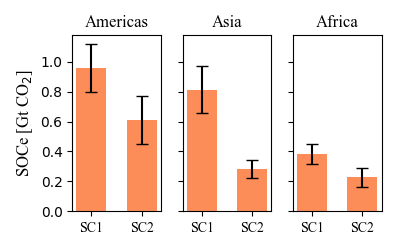
\includegraphics[scale=1]{img/soce}
%			\caption[Ecosystem service values]{}
%			\label{fig:soce}
%		\end{figure}
%
%		\begin{table}[ht]
%			\centering
%			\caption[Soil organic carbon emissions]{Soil organic carbon emissions}
%			\label{tab:soce_tab}
%			\begin{tabular}{lrrrrrrrrr}
%				\hline
%				\multirow{3}{*}{Region} & \multicolumn{3}{c}{SC1}& \multicolumn{3}{c}{SC2} & \multicolumn{3}{c}{SC3} \\
%				& \multicolumn{3}{c}{[Gt CO$_2$]}& \multicolumn{3}{c}{[Gt CO$_2$]} & \multicolumn{3}{c}{[Gt CO$_2$]} \\
%				& min & mean & max & min & mean & max & min & mean & max \\\hline
%				Americas & 0.80 & 0.96 & 1.12 & 0.45 & 0.61 & 0.77 & 0.43 & 0.59 & 0.76 \\
%				Asia & 0.66 & 0.81 & 0.97 & 0.22 & 0.28 & 0.34 & 0.22 & 0.28 & 0.33 \\
%				Africa & 0.32 & 0.39 & 0.45 & 0.17 & 0.23 & 0.29 & 0.16 & 0.23 & 0.29 \\\hline
%			\end{tabular}
%		\end{table}


% ESV
%		\begin{figure}[ht]
%			\centering
%			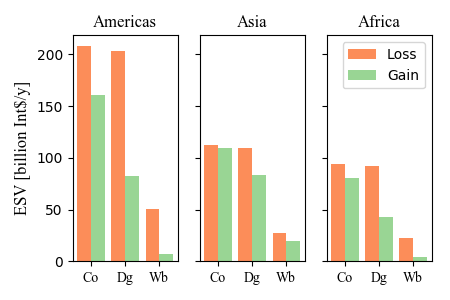
\includegraphics[scale=1]{img/esv}
%			\caption[Ecosystem service values]{}
%			\label{fig:esv}
%		\end{figure}


